%% (Master) Thesis template
% Template version used: v1.4
%
% Largely adapted from Adrian Nievergelt's template for the ADPS
% (lecture notes) project.


%% We use the memoir class because it offers a many easy to use features.
\documentclass[11pt,a4paper,titlepage]{memoir}

%% Packages
%% ========

%% LaTeX Font encoding -- DO NOT CHANGE
\usepackage[OT1]{fontenc}

%% Babel provides support for languages.  'english' uses British
%% English hyphenation and text snippets like "Figure" and
%% "Theorem". Use the option 'ngerman' if your document is in German.
%% Use 'american' for American English.  Note that if you change this,
%% the next LaTeX run may show spurious errors.  Simply run it again.
%% If they persist, remove the .aux file and try again.
\usepackage[english]{babel}

%% Input encoding 'utf8'. In some cases you might need 'utf8x' for
%% extra symbols. Not all editors, especially on Windows, are UTF-8
%% capable, so you may want to use 'latin1' instead.
\usepackage[utf8]{inputenc}

%% This changes default fonts for both text and math mode to use Herman Zapfs
%% excellent Palatino font.  Do not change this.
\usepackage[sc]{mathpazo}

%% The AMS-LaTeX extensions for mathematical typesetting.  Do not
%% remove.
\usepackage{amsmath,amssymb,amsfonts,mathrsfs}

%% NTheorem is a reimplementation of the AMS Theorem package. This
%% will allow us to typeset theorems like examples, proofs and
%% similar.  Do not remove.
%% NOTE: Must be loaded AFTER amsmath, or the \qed placement will
%% break
\usepackage[amsmath,thmmarks]{ntheorem}

%% LaTeX' own graphics handling
\usepackage{graphicx}

%% We unfortunately need this for the Rules chapter.  Remove it
%% afterwards; or at least NEVER use its underlining features.
\usepackage{soul}

%% This allows you to add .pdf files. It is used to add the
%% declaration of originality.
\usepackage{pdfpages}



%% Include movies
\usepackage{movie15} 
%% Some more packages that you may want to use.  Have a look at the
%% file, and consult the package docs for each.
%% See the TeXed file for more explanations

%% [OPT] Multi-rowed cells in tabulars
%\usepackage{multirow}

%% [REC] Intelligent cross reference package. This allows for nice
%% combined references that include the reference and a hint to where
%% to look for it.
\usepackage{varioref}

%% [OPT] Easily changeable quotes with \enquote{Text}
%\usepackage[german=swiss]{csquotes}

%% [REC] Format dates and time depending on locale
\usepackage{datetime}

%% [OPT] Provides a \cancel{} command to stroke through mathematics.
%\usepackage{cancel}

%% [NEED] This allows for additional typesetting tools in mathmode.
%% See its excellent documentation.
\usepackage{mathtools}

%% [ADV] Conditional commands
%\usepackage{ifthen}

%% [OPT] Manual large braces or other delimiters.
%\usepackage{bigdelim, bigstrut}

%% [REC] Alternate vector arrows. Use the command \vv{} to get scaled
%% vector arrows.
\usepackage[h]{esvect}

%% [NEED] Some extensions to tabulars and array environments.
\usepackage{array}

%% [OPT] Postscript support via pstricks graphics package. Very
%% diverse applications.
%\usepackage{pstricks,pst-all}

%% [?] This seems to allow us to define some additional counters.
%\usepackage{etex}

%% [ADV] XY-Pic to typeset some matrix-style graphics
%\usepackage[all]{xy}

%% [OPT] This is needed to generate an index at the end of the
%% document.
%\usepackage{makeidx}

%% [OPT] Fancy package for source code listings.  The template text
%% needs it for some LaTeX snippets; remove/adapt the \lstset when you
%% remove the template content.
\usepackage{listings}
\lstset{language=TeX,basicstyle={\normalfont\ttfamily}}

%% [REC] Fancy character protrusion.  Must be loaded after all fonts.
\usepackage[activate]{pdfcprot}

%% [REC] Nicer tables.  Read the excellent documentation.
\usepackage{booktabs}


%% Our layout configuration.  DO NOT CHANGE.
%% Memoir layout setup

%% NOTE: You are strongly advised not to change any of them unless you
%% know what you are doing.  These settings strongly interact in the
%% final look of the document.

% Dependencies
\usepackage{ETHlogo}

% Turn extra space before chapter headings off.
\setlength{\beforechapskip}{0pt}

\nonzeroparskip
\parindent=0pt
\defaultlists

% Chapter style redefinition
\makeatletter

\if@twoside
  \pagestyle{Ruled}
  \copypagestyle{chapter}{Ruled}
\else
  \pagestyle{ruled}
  \copypagestyle{chapter}{ruled}
\fi
\makeoddhead{chapter}{}{}{}
\makeevenhead{chapter}{}{}{}
\makeheadrule{chapter}{\textwidth}{0pt}
\copypagestyle{abstract}{empty}

\makechapterstyle{bianchimod}{%
  \chapterstyle{default}
  \renewcommand*{\chapnamefont}{\normalfont\Large\sffamily}
  \renewcommand*{\chapnumfont}{\normalfont\Large\sffamily}
  \renewcommand*{\printchaptername}{%
    \chapnamefont\centering\@chapapp}
  \renewcommand*{\printchapternum}{\chapnumfont {\thechapter}}
  \renewcommand*{\chaptitlefont}{\normalfont\huge\sffamily}
  \renewcommand*{\printchaptertitle}[1]{%
    \hrule\vskip\onelineskip \centering \chaptitlefont\textbf{\vphantom{gyM}##1}\par}
  \renewcommand*{\afterchaptertitle}{\vskip\onelineskip \hrule\vskip
    \afterchapskip}
  \renewcommand*{\printchapternonum}{%
    \vphantom{\chapnumfont {9}}\afterchapternum}}

% Use the newly defined style
\chapterstyle{bianchimod}

\setsecheadstyle{\Large\bfseries\sffamily}
\setsubsecheadstyle{\large\bfseries\sffamily}
\setsubsubsecheadstyle{\bfseries\sffamily}
\setparaheadstyle{\normalsize\bfseries\sffamily}
\setsubparaheadstyle{\normalsize\itshape\sffamily}
\setsubparaindent{0pt}

% Set captions to a more separated style for clearness
\captionnamefont{\sffamily\bfseries\footnotesize}
\captiontitlefont{\sffamily\footnotesize}
\setlength{\intextsep}{16pt}
\setlength{\belowcaptionskip}{1pt}

% Set section and TOC numbering depth to subsection
\setsecnumdepth{subsection}
\settocdepth{subsection}

%% Titlepage adjustments
\pretitle{\vspace{0pt plus 0.7fill}\begin{center}\HUGE\sffamily\bfseries}
\posttitle{\end{center}\par}
\preauthor{\par\begin{center}\let\and\\\Large\sffamily}
\postauthor{\end{center}}
\predate{\par\begin{center}\Large\sffamily}
\postdate{\end{center}}

\def\@advisors{}
\newcommand{\advisors}[1]{\def\@advisors{#1}}
\def\@department{}
\newcommand{\department}[1]{\def\@department{#1}}
\def\@thesistype{}
\newcommand{\thesistype}[1]{\def\@thesistype{#1}}

\renewcommand{\maketitlehooka}{\noindent\ETHlogo[2in]}

\renewcommand{\maketitlehookb}{\vspace{1in}%
  \par\begin{center}\Large\sffamily\@thesistype\end{center}}

\renewcommand{\maketitlehookd}{%
  \vfill\par
  \begin{flushright}
    \sffamily
    \@advisors\par
    \@department, ETH Z\"urich
  \end{flushright}
}

\checkandfixthelayout

\setlength{\droptitle}{-48pt}

\makeatother

% This defines how theorems should look. Best leave as is.
\theoremstyle{plain}
\setlength\theorempostskipamount{0pt}

%%% Local Variables:
%%% mode: latex
%%% TeX-master: "thesis"
%%% End:


%% Theorem environments.  You will have to adapt this for a German
%% thesis.
%% Theorem-like environments

%% This can be changed according to language. You can comment out the ones you
%% don't need.

\numberwithin{equation}{chapter}

%% German theorems
%\newtheorem{satz}{Satz}[chapter]
%\newtheorem{beispiel}[satz]{Beispiel}
%\newtheorem{bemerkung}[satz]{Bemerkung}
%\newtheorem{korrolar}[satz]{Korrolar}
%\newtheorem{definition}[satz]{Definition}
%\newtheorem{lemma}[satz]{Lemma}
%\newtheorem{proposition}[satz]{Proposition}

%% English variants
\newtheorem{theorem}{Theorem}[chapter]
\newtheorem{example}[theorem]{Example}
\newtheorem{remark}[theorem]{Remark}
\newtheorem{corollary}[theorem]{Corollary}
\newtheorem{definition}[theorem]{Definition}
\newtheorem{lemma}[theorem]{Lemma}
\newtheorem{proposition}[theorem]{Proposition}

%% Proof environment with a small square as a "qed" symbol
\theoremstyle{nonumberplain}
\theorembodyfont{\normalfont}
\theoremsymbol{\ensuremath{\square}}
\newtheorem{proof}{Proof}
%\newtheorem{beweis}{Beweis}


%% Helpful macros.
%% Custom commands
%% ===============

%% Special characters for number sets, e.g. real or complex numbers.
\newcommand{\C}{\mathbb{C}}
\newcommand{\K}{\mathbb{K}}
\newcommand{\N}{\mathbb{N}}
\newcommand{\Q}{\mathbb{Q}}
\newcommand{\R}{\mathbb{R}}
\newcommand{\Z}{\mathbb{Z}}
\newcommand{\X}{\mathbb{X}}

%% Fixed/scaling delimiter examples (see mathtools documentation)
\DeclarePairedDelimiter\abs{\lvert}{\rvert}
\DeclarePairedDelimiter\norm{\lVert}{\rVert}

%% Use the alternative epsilon per default and define the old one as \oldepsilon
\let\oldepsilon\epsilon
\renewcommand{\epsilon}{\ensuremath\varepsilon}

%% Also set the alternate phi as default.
\let\oldphi\phi
\renewcommand{\phi}{\ensuremath{\varphi}}



%% Make document internal hyperlinks wherever possible. (TOC, references)
%% This MUST be loaded after varioref, which is loaded in 'extrapackages'
%% above.  We just load it last to be safe.
\usepackage[linkcolor=black,colorlinks=true,citecolor=black,filecolor=black]{hyperref}


%% Document information
%% ====================

\title{2D Incompressible Flow Solver}
\author{Omar Suleman}
\thesistype{Fundamentals of CFD \\ Semester Project}
\advisors{Instructor: Prof.\ Dr. Andreas Haselbacher}
\department{Dep. of Mechanical and Process Engineering}
\date{May 15, 2014}

\begin{document}

\frontmatter

%% Title page is autogenerated from document information above.  DO
%% NOT CHANGE.
\begin{titlingpage}
  \calccentering{\unitlength}
  \begin{adjustwidth*}{\unitlength-24pt}{-\unitlength-24pt}
    \maketitle
  \end{adjustwidth*}
\end{titlingpage}

%% The abstract of your thesis.  Edit the file as needed.
\begin{abstract}

This report discusses the development of a CFD program for solving 2D incompressible flow, using the Stream-Vorticity formulations of the Navier Stokes equations.  The code uses $2^{nd}$ order, centered spatial discretizations, and an explicit first order temporal discretization.  The SOR and ADI method are both implemented as iterative solvers for the Poisson Equation, then compared in terms of program run time.  An order verification study is performed on the spatial discretizations used.  The program is tested by simulating a Shear Driven Cavity Flow problem, and the results are compared with a similar study done previously by Ghia Et. Al. \cite{Ghia1982}.  Finally, a grid refinement study is performed to observe the effects of a changing grid size on the numerical solution.  


\end{abstract}


%% TOC with the proper setup, do not change.
\cleartorecto
\tableofcontents
\mainmatter

%% Your real content!
\chapter{Introduction}

This report outlines the background physics, numerical methods and validation of a CFD program developed in C++ to solve the 2D incompressible Navier Stokes equation, using the Steam-Vorticity formulation.


\section{Governing Equations}
\label{sec:gov_eqs}

The Vorticity equation \ref{eq:vorticity} is obtained by taking the curl of the incompressible Navier Stokes momentum equations.  In doing so, the pressure term is eliminated from these equations.  In 2D, the problem is greatly simplified to only two unknowns, because the vorticity only has one component.  The continuity equation can be written in terms of the other unknown, in the Stream Function \ref{eq:poisson}.  


\begin{equation}
\label{eq:poisson} 
\frac{\delta^2 \overline{\psi}}{\delta \overline{x}^2} + \frac{\delta^2 \overline{\psi}}{\delta \overline{y}^2} = -\overline{\zeta}
\end{equation}

\begin{equation}
\label{eq:vorticity} 
              \frac { \delta \overline{\zeta}}{\delta \overline{t}} + 
\overline{u} \frac{\delta \overline{\zeta}}{\delta \overline{x}} + 
\overline{v} \frac{\delta \overline{\zeta}}{\delta \overline{y}} = 
\frac{1}{Re} \Big(\frac{\delta^2 \overline{\zeta}}{\delta \overline{x}^2} + 
\frac{\delta^2 \overline{\zeta}}{\delta \overline{y}^2} \Big)
\end{equation}




\noindent\begin{minipage}{.5\linewidth}
\begin{equation}
\label{eq:u}        
\overline{u} =  \frac{\delta \overline{\psi}}{\delta \overline{y}} 
\end{equation}
\end{minipage}%
\begin{minipage}{.5\linewidth}
\begin{equation}
\label{eq:v} 
\overline{v} = - \frac{\delta \overline{\psi}}{\delta \overline{x}}
\end{equation}
\end{minipage}


\section{Test Case}
\label{sec:test_case}

The problem being simulated to validate the model is shear driven cavity flow.  This problem involves laminar flow of an incompressible, viscous fluid in a square cavity, where all the walls are stationary, except for the top wall moving at a constant velocity.  The steady state data from this study will be compared to a previous study of this problem by Ghia Et. Al. \cite{Ghia1982}.

	\subsection{Boundary Conditions}

For all the walls, the velocity normal to the wall is zero because the mass flux at the wall must be zero, since no mass leaves or enters the control volume.  Based on this condition and Equations \ref{eq:u} and \ref{eq:v}, $\psi|_{wall}$ is constant in the direction parallel to the walls. Since all the walls are connected, and $\psi|_{wall}$ is constant along each wall, $\psi|_{wall}$ is the same constant for all walls. This constant was arbitrarily set to zero; it's value will not affect the vorticity or velocity field, since these quantities are functions of the derivative of $\psi$, and not $\psi$ itself. 

\begin{equation}
\label{eq:bc_psi} 
\psi\Big|_{wall} = c = 0
\end{equation}

The Poisson Equation \ref{eq:poisson} can be simplified knowing that $\psi$ is constant when moving along the wall.  This simplification is shown in Equations \ref{eq:zeta_horz_wall} and \ref{eq:zeta_vert_wall}.

\begin{equation}
\label{eq:zeta_horz_wall} 
\overline{\zeta}(x,0) = \overline{\zeta}(x,1)  =
- \frac{\delta^2 \overline{\psi}}{\delta \overline{y}^2} 
\end{equation}

\begin{equation}
\label{eq:zeta_vert_wall} 
\overline{\zeta}(0,y) = \overline{\zeta}(1,y)  =
- \frac{\delta^2 \overline{\psi}}{\delta \overline{x}^2} 
\end{equation}


The velocity parallel to the wall is equal to the wall velocity, to satisfy the no slip boundary condition.  This is expressed in Equations \ref{eq:v_stationary} to \ref{eq:v_moving}.  This second boundary condition will be applied to Equations \ref{eq:zeta_horz_wall} and \ref{eq:zeta_vert_wall} when the equations are discretized, to create a boundary condition for $\zeta$.

\begin{equation}
\label{eq:v_stationary} 
\overline{v}(0,y,t) = \overline{v}(1,y,t) = \overline{u}(x,0,t) = 0
\end{equation}

\begin{equation}
\label{eq:v_moving} 
\overline{u}(x,1,t) = \frac{u}{u_{ref}} = 1
\end{equation}




	\subsection{Initial Conditions}

Since only the steady state data is of interest, the initial conditions can be arbitrary because the solutions will converge to the same steady state values, regardless of initial conditions.  The initial conditions selected are given in Equation \ref{eq:ic_zeta} and \ref{eq:ic_psi}.

\begin{equation}
\label{eq:ic_zeta} 
\overline{\zeta}(x,y,0) = 0
\end{equation}

\begin{equation}
\label{eq:ic_psi} 
\overline{\psi}(x,y,0) = 0
\end{equation}	
	


\chapter{Methods}

\section{Program Structure}
\label{sec:prog_struct}

The program is implemented in C++, using object orientated programming.  The goal was to make the structure modular so that in future, a variety of problems could be solved on many different style grids, in higher dimensions.

The spatial domain is discretized and stored as a grid object.  The grid class holds a fluid element object for each discrete point in the spatial domain, as well as any parameters specific to that particular grid.  The fluid element holds all variables of interest at that particular point in space, as well as its position in space.  All the variables stored at the fluid element object level are non-dimensionalized by the reference values stored in the grid object.  Since all the variables in the governing equations are stored in the fluid element, the equations being solved are non-dimensional.  

The data is output using the Visualization Toolkit from Kitware.  All the scalar variables, and the velocity fields are written to a VTK file at specified dump period.  The data can be directly opened in ParaView and visualized directly.  Additionally, a text file is written out at the end of each simulation and contains a text file with the u-velocity component along the vertical centerline, and the v-velocity component along the horizontal centerline.  The program has no runtime arguments.  All the parameters are specified in the Main.cpp file. For instruction on compiling and executing the program, refer to the readme.txt in the main project folder.

\section{Numerical Discretization}
\label{sec:num_disc}

The numerical schemes used to discretize the governing equations presented in Section \ref{sec:gov_eqs} are provided below.

	\subsection{Spacial Discretization}

The first and second spacial derivatives are discretized with second order accurate, centered schemes.  The equations for the first order derivatives are given in Equation \ref{eq:first_deriv_x} and Equation \ref{eq:first_deriv_y}.  The equations for the second order derivatives are given in Equation \ref{eq:second_deriv_x} and Equation \ref{eq:second_deriv_y}.

\begin{equation} 
\label{eq:first_deriv_x}
\frac{\partial u}{\partial x}\bigg|_{i,j} = \frac{u_{ i+1,j} - u_{ i-1,j}}{2\Delta x} 
\end{equation}

\begin{equation} 
\label{eq:first_deriv_y}
\frac{\partial u}{\partial y}\bigg|_{i,j} = \frac{u_{ i,j+1} - u_{ i,j-1}}{2\Delta y}
\end{equation}

\begin{equation} 
\label{eq:second_deriv_x}
\frac{\partial^2 u}{\partial x^2}\bigg|_{i,j} = \frac{u_{ i+1,j} - 2 u_{ i,j} + u_{ i-1,j} }{{\Delta x}^2} 
\end{equation}

\begin{equation} 
\label{eq:second_deriv_y}
\frac{\partial^2 u}{\partial x^2}\bigg|_{i,j} = \frac{u_{ i,j+1} - 2 u_{ i,j} + u_{ i,j-1} }{{\Delta x}^2} 
\end{equation}

The derivative operator can be applied to any variable stored in the fluid element class.  Note that this derivative approximation is only valid for constant $\Delta x$ and $\Delta y$.


	\subsection{Temporal Discretization}

The temporal derivative is discretized with the explicit, first order accurate Euler scheme, and used to solve for the next time step, as shown in Equation \ref{eq:time_deriv}

\begin{equation}
\label{eq:time_deriv}
u_{i,j}^{n+1} = u_{i,j}^{n} + \frac{\partial u}{\partial t}\bigg|_{i,j}^{n} \Delta t
\end{equation}

The approximation in Equation \ref{eq:time_deriv} is only first order accurate, unlike the spacial approximation.  

\section{Implementation of Boundary Conditions}

	
The boundary condition for $\psi$, given in Equation \ref{eq:bc_psi}, can be directly implemented.  The boundary condition for $\zeta$ must be extracted from the no slip boundary conditions, in Equations \ref{eq:v_stationary} and \ref{eq:v_moving}, and applied to the simplified Poisson Equations in \ref{eq:zeta_horz_wall} and \ref{eq:zeta_vert_wall}. These equations are discretized with the schemes given in Section \ref{sec:num_disc}, and displayed in Equations \ref{eq:zeta_bot_wall_disc} to \ref{eq:v_right_disc}.  Also note that \ $\psi|_{wall}$ was set to zero in Equation \ref{eq:bc_psi}, allowing further simplification of the discrete equations.  Using these discrete equations, a boundary condition expression for $\zeta$ was obtained and implemented into the solver; these equations are displayed in \ref{eq:bc_zeta_bot} to \ref{eq:bc_zeta_right}.

\begin{equation}
\label{eq:zeta_bot_wall_disc} 
\overline{\zeta}_{i,0} = - \frac{\psi_{ i,1} - 2 \psi_{ i,0} + \psi_{ i,-1} }{{\Delta y}^2}
= \frac{\psi_{ i,1} + \psi_{ i,-1} }{{\Delta y}^2}
\end{equation}

\begin{equation}
\label{eq:zeta_top_wall_disc} 
\overline{\zeta}_{i,ny-1} = - \frac{\psi_{ i,ny} - 2 \psi_{ i,ny-1} + \psi_{ i,ny-2} }{{\Delta y}^2} = - \frac{\psi_{ i,ny} + \psi_{ i,ny-2} }{{\Delta y}^2}
\end{equation}

\begin{equation}
\label{eq:zeta_left_wall_disc} 
\overline{\zeta}_{0,j} = - \frac{\psi_{1,j} - 2 \psi_{0,j} + \psi_{-1,j} }{{\Delta x}^2} 
= - \frac{\psi_{1,j} + \psi_{-1,j} }{{\Delta x}^2} 
\end{equation}

\begin{equation}
\label{eq:zeta_right_wall_disc} 
\overline{\zeta}_{nx-1,j} = - \frac{\psi_{nx,j} - 2 \psi_{nx-1,j} + \psi_{nx-2,j} }{{\Delta x}^2} =  - \frac{\psi_{nx,j} + \psi_{nx-2,j} }{{\Delta x}^2} 
\end{equation}



\begin{equation}
\label{eq:v_bot_disc} 
\frac{\psi_{ i,1} - \psi_{ i,-1}}{2\Delta y} = 0
\end{equation}

\begin{equation}
\label{eq:v_top_disc} 
\frac{\psi_{ i,ny} - \psi_{ i,ny-2}}{2\Delta y} = 1
\end{equation}



\begin{equation}
\label{eq:v_left_disc} 
\frac{\psi_{1,j} - \psi_{-1,j}}{2\Delta x} = 0
\end{equation}

\begin{equation}
\label{eq:v_right_disc} 
\frac{\psi_{nx,j} - \psi_{nx-2,j}}{2\Delta x} = 0
\end{equation}




\begin{equation}
\label{eq:bc_zeta_bot} 
\zeta_{i,0} = 2\frac{\psi_{i,1}}{\Delta y}
\end{equation}

\begin{equation}
\label{eq:bc_zeta_top} 
\zeta_{i,ny-1} = 2\Big( \frac{\psi_{i,ny-2}}{\Delta y}  - \Delta y \Big)
\end{equation}



\begin{equation}
\label{eq:bc_zeta_left} 
\zeta_{0,j} = 2\frac{\psi_{1,j}}{\Delta y}
\end{equation}

\begin{equation}
\label{eq:bc_zeta_right} 
\zeta_{nx-1,j} = 2\frac{\psi_{nx-2,j}}{\Delta x}
\end{equation}



\section{Solution Algorithms}
\label{sec:sol_algo}

To solve the Poisson equation, an iterative solver was required.  Two different algorithms were used, and are detailed below.

	\subsection{Successive Over-Relaxation Method}
The Successive Over-Relaxation (SOR) Method iterates through the grid, and explicitly solves for the value of the variable being solved, so that it satisfies the governing equation.  Next, the value of the variable is updated on the grid using a linear combination of the old and new value.  This calculation is shown for one single point on the grid in Equation \ref{eq:poisson_sor1} and \ref{eq:poisson_sor2}.  This process is repeated until the the difference between $\psi_{i,j,new}$ and $\psi_{i,j}$ is less than a specified tolerance, everywhere in the grid.


\begin{equation}
\label{eq:poisson_sor1} 
\psi_{i,j,new} = \frac{(\psi_{i+1,j} + \psi_{i-1,j}) + (\psi_{i,j+1} + \psi_{i,j-1})\big( \frac{\Delta x}{\Delta y} \big) ^2 + \zeta_{i,j}  (\Delta x)^2}{2 \big( 1 + (\frac{\Delta x}{\Delta y})^2 \big)}
\end{equation}


\begin{equation}
\label{eq:poisson_sor2} 
\psi_{i,j} = \omega \psi_{i,j,new} + (1 - \omega) \psi_{i,j,old} 
\end{equation}



	\subsection{Alternating Direction Implicit Method}

The ADI Method is an implicit numerical scheme for temporal discretization of linear equations.  Time steps are subdivided into smaller steps (2 steps for 2D ect.), and at each partial step, only terms in a single dimension are represented implicitly.  After one partial time step, the terms previously represented implicitly, are represented explicitly, and the terms in the next dimension are represented implicitly.  In doing so, a complicated block tri-diagonal linear system is avoided, and instead, the linear system being solve is tri-diagonal.  This is cheaper computationally to solve than a tri-diagonal system, and this implicit scheme has favorable stability properties, allowing larger time steps.

A time derivative term was added to the Poisson Equation \ref{eq:poisson}, and the Alternating Direction Implicit (ADI) Method was used to solve for the steady state solution of this equation.  The modified Poisson Equation is given in \ref{eq:poisson_dt}.  A variable time step is used for fast convergence, and is defined in equations \ref{eq:rho_adi} to \ref{eq:p_max}.  The resulting tri-diagonal system was solved with the Thomas algorthm for tri-diagonal matrices.


%The  discrete equation to be solved and the resulting tri-diagonal system is shown in..  The time step was incremented according to.. until steady state was reached.  Steady state is defined as..


\begin{equation}
\label{eq:poisson_dt} 
\frac{\delta \overline{\psi}}{\delta \overline{t}} =
\frac{\delta^2 \overline{\psi}}{\delta \overline{x}^2} + \frac{\delta^2 \overline{\psi}}{\delta \overline{y}^2} + \overline{\zeta}
\end{equation}

\begin{equation}
\label{eq:poisson_adi_1} 
 \overline{\psi}_{i,j}^{n+\frac{1}{2}} = \overline{\psi}_{i,j}^{n} +
 \frac{Re \Delta t}{{\Delta x}^2} \big(
 \overline{\psi}_{i+1,j}^{n+\frac{1}{2}} - 2 \overline{\psi}_{i,j}^{n+\frac{1}{2}} + \overline{\psi}_{i-1,j}^{n+\frac{1}{2}}
 \big)  + 
 \frac{Re \Delta t}{{\Delta y}^2} \big(
 \overline{\psi}_{i,j+1}^{n} - 2 \overline{\psi}_{i,j}^{n} + \overline{\psi}_{i,j-1}^{n}
 \big) + \zeta_{i,j}^{n} \Delta t
\end{equation}




\begin{equation}
\label{eq:poisson_adi_2} 
 \overline{\psi}_{i,j}^{n+1} = \overline{\psi}_{i,j}^{n+\frac{1}{2}} +
 \frac{Re \Delta t}{{\Delta x}^2} \big(
 \overline{\psi}_{i+1,j}^{n+\frac{1}{2}} - 2 \overline{\psi}_{i,j}^{n+\frac{1}{2}} + \overline{\psi}_{i-1,j}^{n+\frac{1}{2}}
 \big) + 
 \frac{Re \Delta t}{{\Delta y}^2} \big(
 \overline{\psi}_{i,j+1}^{n+1} - 2 \overline{\psi}_{i,j}^{n+1} + \overline{\psi}_{i,j-1}^{n+1}
 \big) + \zeta_{i,j}^{n+\frac{1}{2}} \Delta t
\end{equation}


\begin{equation}
\label{eq:rho_adi} 
\rho = \frac{{\Delta x}^2}{\Delta t}
\end{equation}

\begin{equation}
\label{eq:rho_opt} 
\rho  = 4\cos^2\big(\frac{\pi dx}{2}\big)\tan^2\big(\frac{\pi dx}{2}\big)^{\frac{(2p-1)}{2p_{max}}}
\end{equation}

\begin{equation}
\label{eq:p_max} 
p = 1,2 .. p_{max},1,2..p_{max} = \frac{\log10(\tan^2(\frac{\pi dx}{2}))}{2\log10(\sqrt2 - 1)}..
\end{equation}

\chapter{Results}



\section{Order Verification Study}
\label{sec:ord_ver_std}

	\subsection{Spacial Discretization}
	\label{sec:s_disc}
A grid refinement study was performed to verify the order of accuracy of the spatial discretizations discussed in Section \ref{sec:num_disc}.  In order to determine the error of the approximations, The Method of Manufactured Solutions was implemented.  A manufactured solution was selected, $\psi_{manu}$, and the analytic right hand side of the corresponding numerical scheme was computed.  The analytic right hand side was used in the numerical scheme, to compute a numerical solution, $\psi_{num}$, that satisfied the numerical scheme to a specified tolerance.  A tolerance of $10^{-12}$ was selected to ensure that the error owing from this tolerance would be negligible in comparison to the discretization error.  The total error could then be computed from Equation \ref{eq:tot_error}.


\begin{equation}
\label{eq:tot_error}
\epsilon = |(\psi_{manu} - \psi_{num})|
\end{equation}


Using Equation \ref{eq:tot_error}, the error for each point in a specific size grid was computed to determine the maximum error, $\epsilon_{max}$.  The maximum error was compared for different grid sizes, and the results are plotted on a log scale in Figure \ref{fig:ovs_sd}.  The dashed vertical lines indicate the minimum and maximum grid spacing that the numerical schemes will be implemented on.

\begin{figure}[h!]
\center
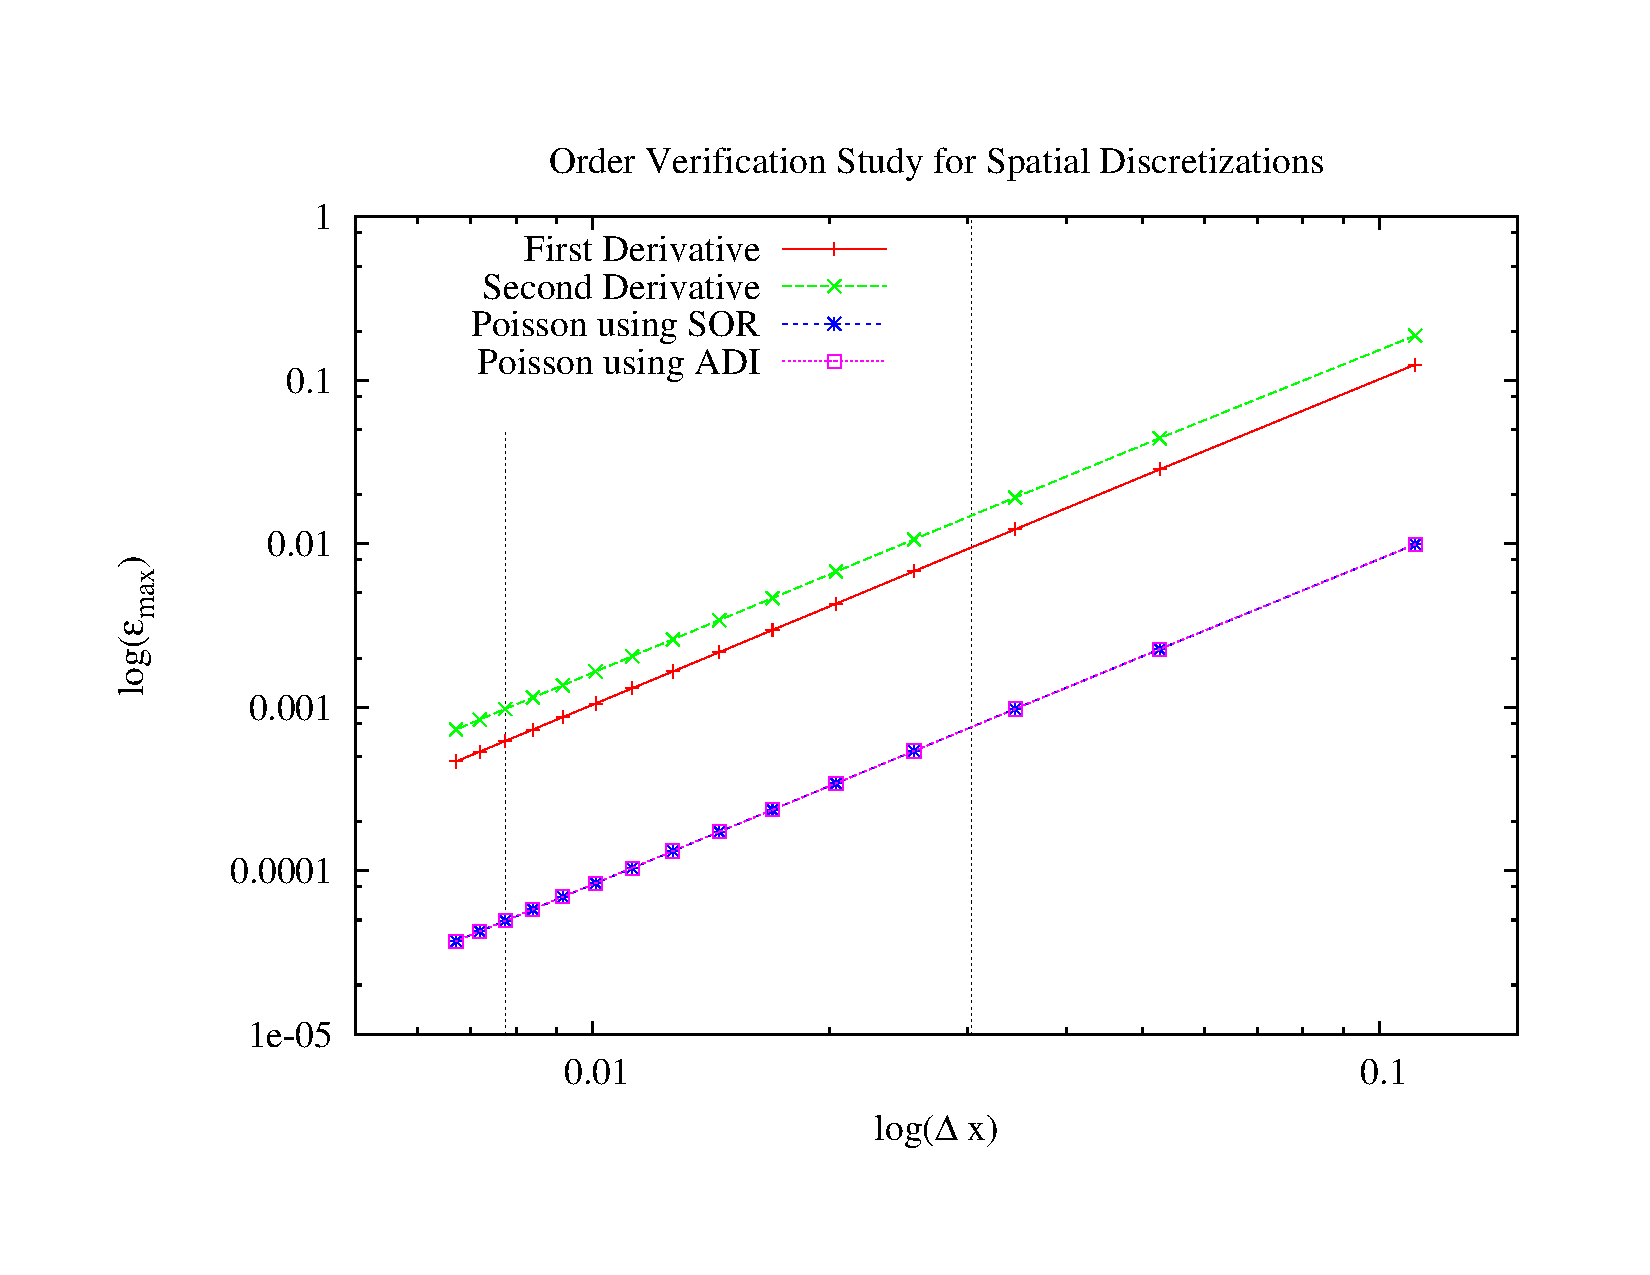
\includegraphics[width=0.9\textwidth]{plots/ovs_sd}
\caption{Maximum numerical error as a function of grid spacing for spatial discretizations, plotted on a log-log scale.}
\label{fig:ovs_sd}
\end{figure}

Using the plots in Figure \ref{fig:ovs_sd}, a linear curve was fit to the data, and the result are summarized in Table \ref{tab:ovs_sd}.  The slope of all the curves is approximately 2, therefore the maximum error in the grid is proportional to the square of the grid spacing, as shown in Proposition \ref{prop:log_slope}, and is consistent with the numerical schemes selected.  It can also be stated that for the selected grid sizes of interest for this study, the numerical error is mainly dominated by discretization error.


\begin{table}
\center
\caption{Summary of Slope Data for Figure \ref{fig:ovs_sd}}
\label{tab:ovs_sd}

\begin{tabular}{l c r}
\hline
Numerical Disc. & Slope & Error \\
\hline 
\hline 
$1^{st}$ Derivative & 1.99461 & $\pm$ 0.001142 \\
$1^{st}$ Derivative & 1.98334 & $\pm$ 0.003548 \\
Poisson w/ SOR      & 1.99383 & $\pm$ 0.001311 \\
Poisson w/ ADI      & 1.99384 & $\pm$ 0.001312 \\
\hline  
\end{tabular}
\end{table}



\begin{proposition}
\label{prop:log_slope}
  The slope of the log plot gives the power of the relationship between the two plotted variables.
\end{proposition}

\begin{proof}
  \begin{displaymath}
    \log(y) = a \log(x) + b \\ \\
    e^{\log(y)} = e^{a \log(x) + b } \\ \\
    y = c x^a \\ \\
    y  \propto  x^a \\     
  \end{displaymath}

\end{proof}

	\subsection{Temporal Discretization}
	\label{sec:t_disc}

A first order accurate temporal discretization was selected for these simulations because only steady state data was required, and the temporal discretization should have no effect on these results.  An order verification study wasn't performed on the temporal discretization, but instead two more simulations were run using two different time steps, to ensure that the steady state results were indifferent to changes in time step.  Unfortunately, some of the numerical precision was lost when the data was written out to file with only 7 decimal places of precision. The only conclusion that can be drawn is that the results were indifferent to 7 decimal places of precision.  

%NO INFO ADDED WITH THESE PLOTS. OMIT
%The data from this study is plotted in Figure \ref{fig:cfl_u} and \ref{fig:cfl_v}.
%
%\begin{figure}[h!]
%\label{fig:cfl_u}
%\center
%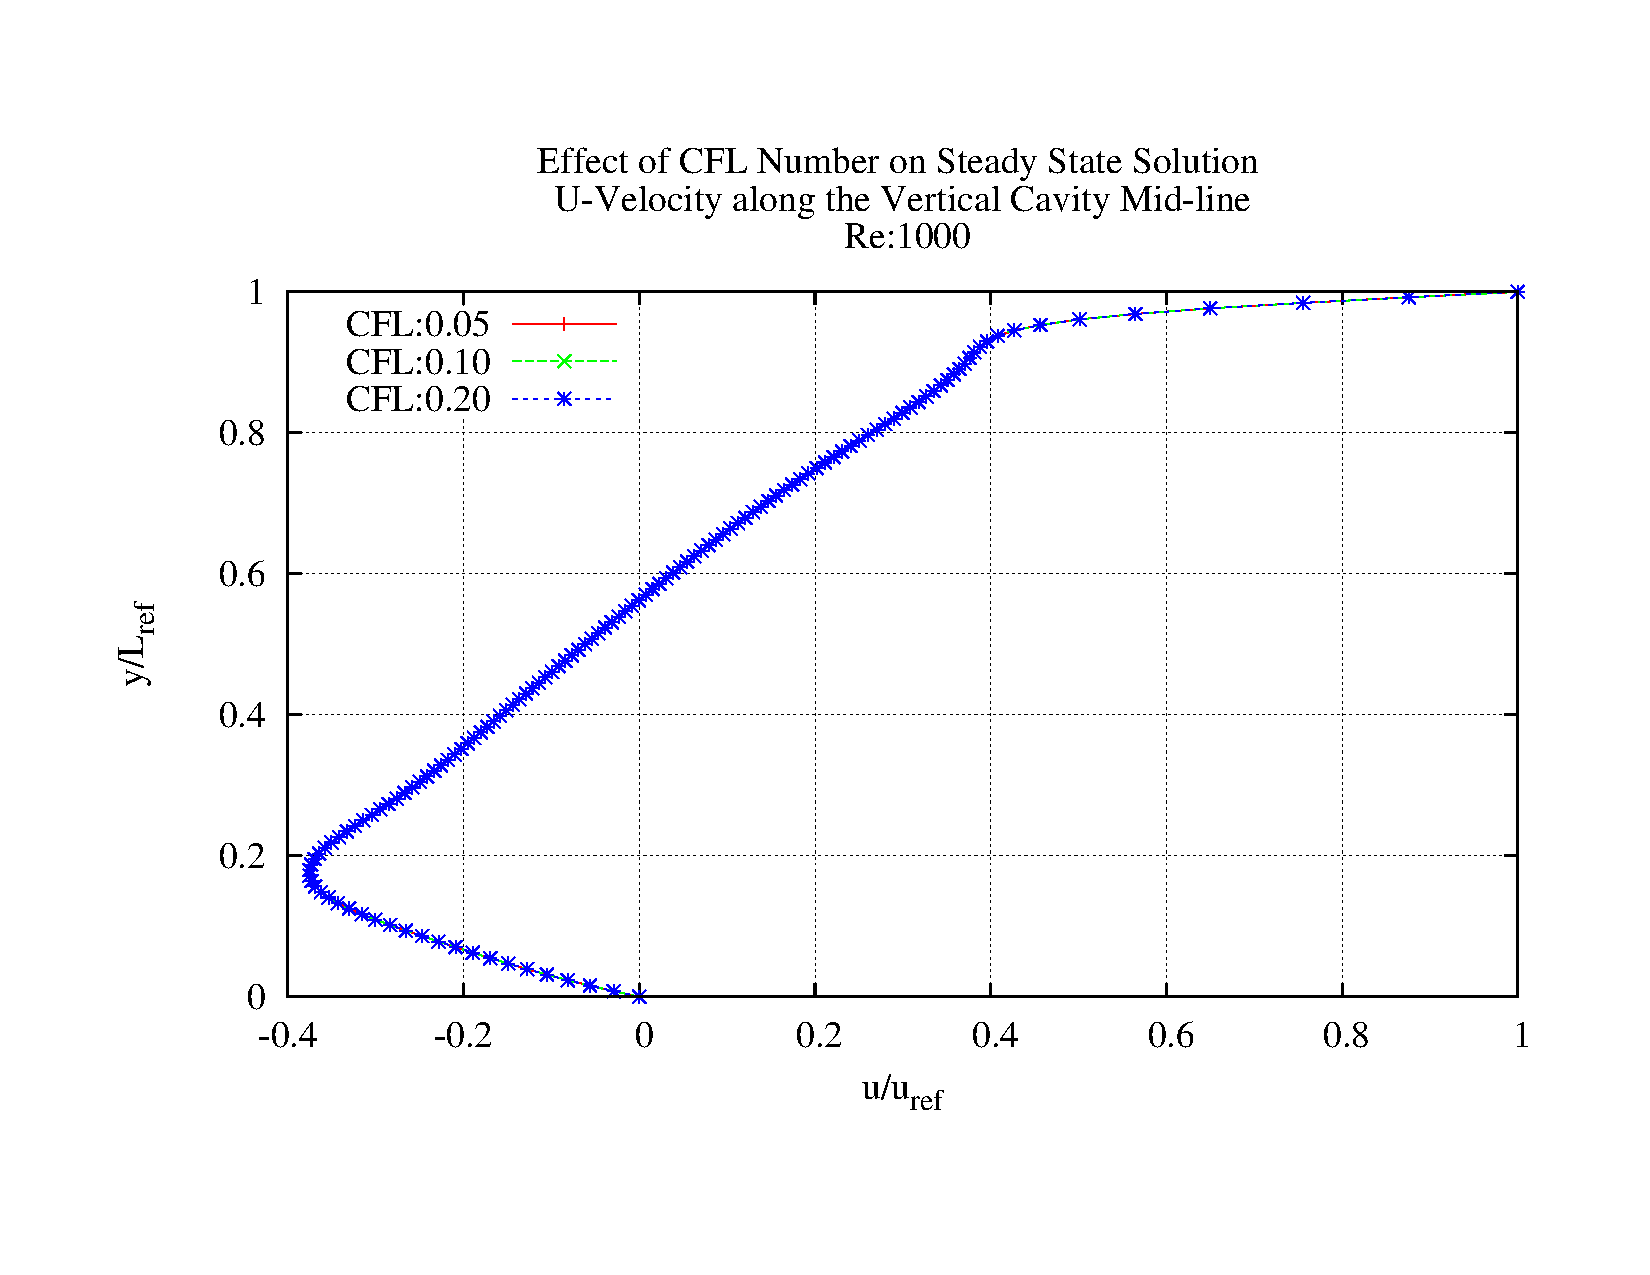
\includegraphics[width=0.9\textwidth]{plots/cfl_u}
%\caption{Steady state u-velocity as a function of y, along the vertical cavity mid-line, for 3 different CFL numbers, at Re:1000.}
%\end{figure}
%
%\begin{figure}[h!]
%\label{fig:cfl_v}
%\center
%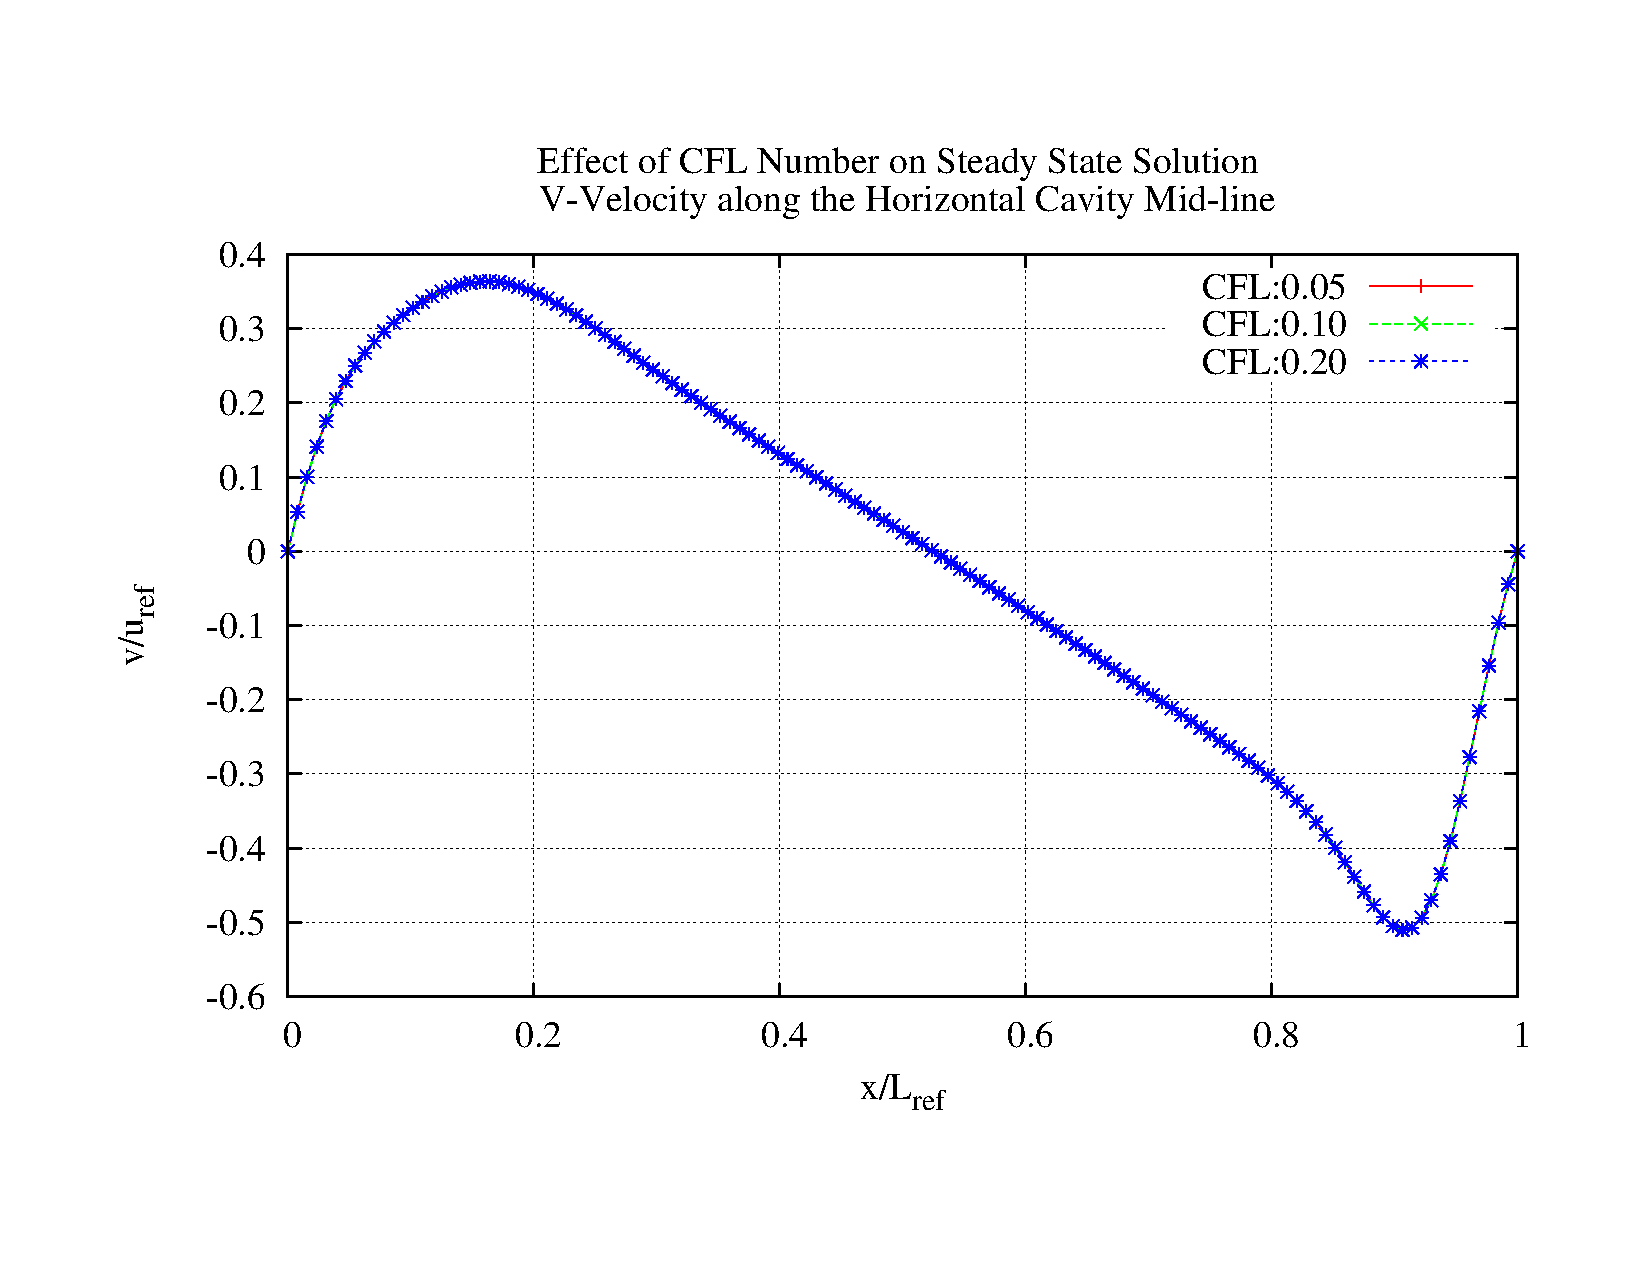
\includegraphics[width=0.9\textwidth]{plots/cfl_v}
%\caption{Steady state v-velocity as a function of x, along the horizontal cavity mid-line, for 3 different CFL numbers, at Re:1000.}
%\end{figure}
%
Additionally, instabilities were observed for a CFL number of 0.5, and the solution failed to converge. A stability analysis was not performed for the forward time, central space (FTCS) scheme implemented, so no comments can be made on this result.  The largest CFL number selected, that leads to stable solutions is 0.2.  There is very little resolution on where the stability limit is; the stability limit is somewhere between $0.2 < CFL < 0.5$.

%A video of the observed instabilities is available in Appendix /ref{app:instability}. 

\section{Optimizing Solution Algorithm}
\label{sec:opt_sol_alg}


	\subsection{Selection of Residual Tolerance}
	\label{sec:res_tol}

The residual tolerance was selected to be as large as possible, without compromising the accuracy of the numerical schemes selected.  This was done by varying the tolerance, performing an order verification study, as described in Section \ref{sec:ord_ver_std}, and observing the effect of tolerance on the solutions order of accuracy.  This process is shown, for both the SOR and ADI solvers, in Figures \ref{fig:rts} and \ref{fig:rta}.  The vertical lines correspond to the fine, medium and coarse grid respectively.

\begin{figure}[h!]
\center
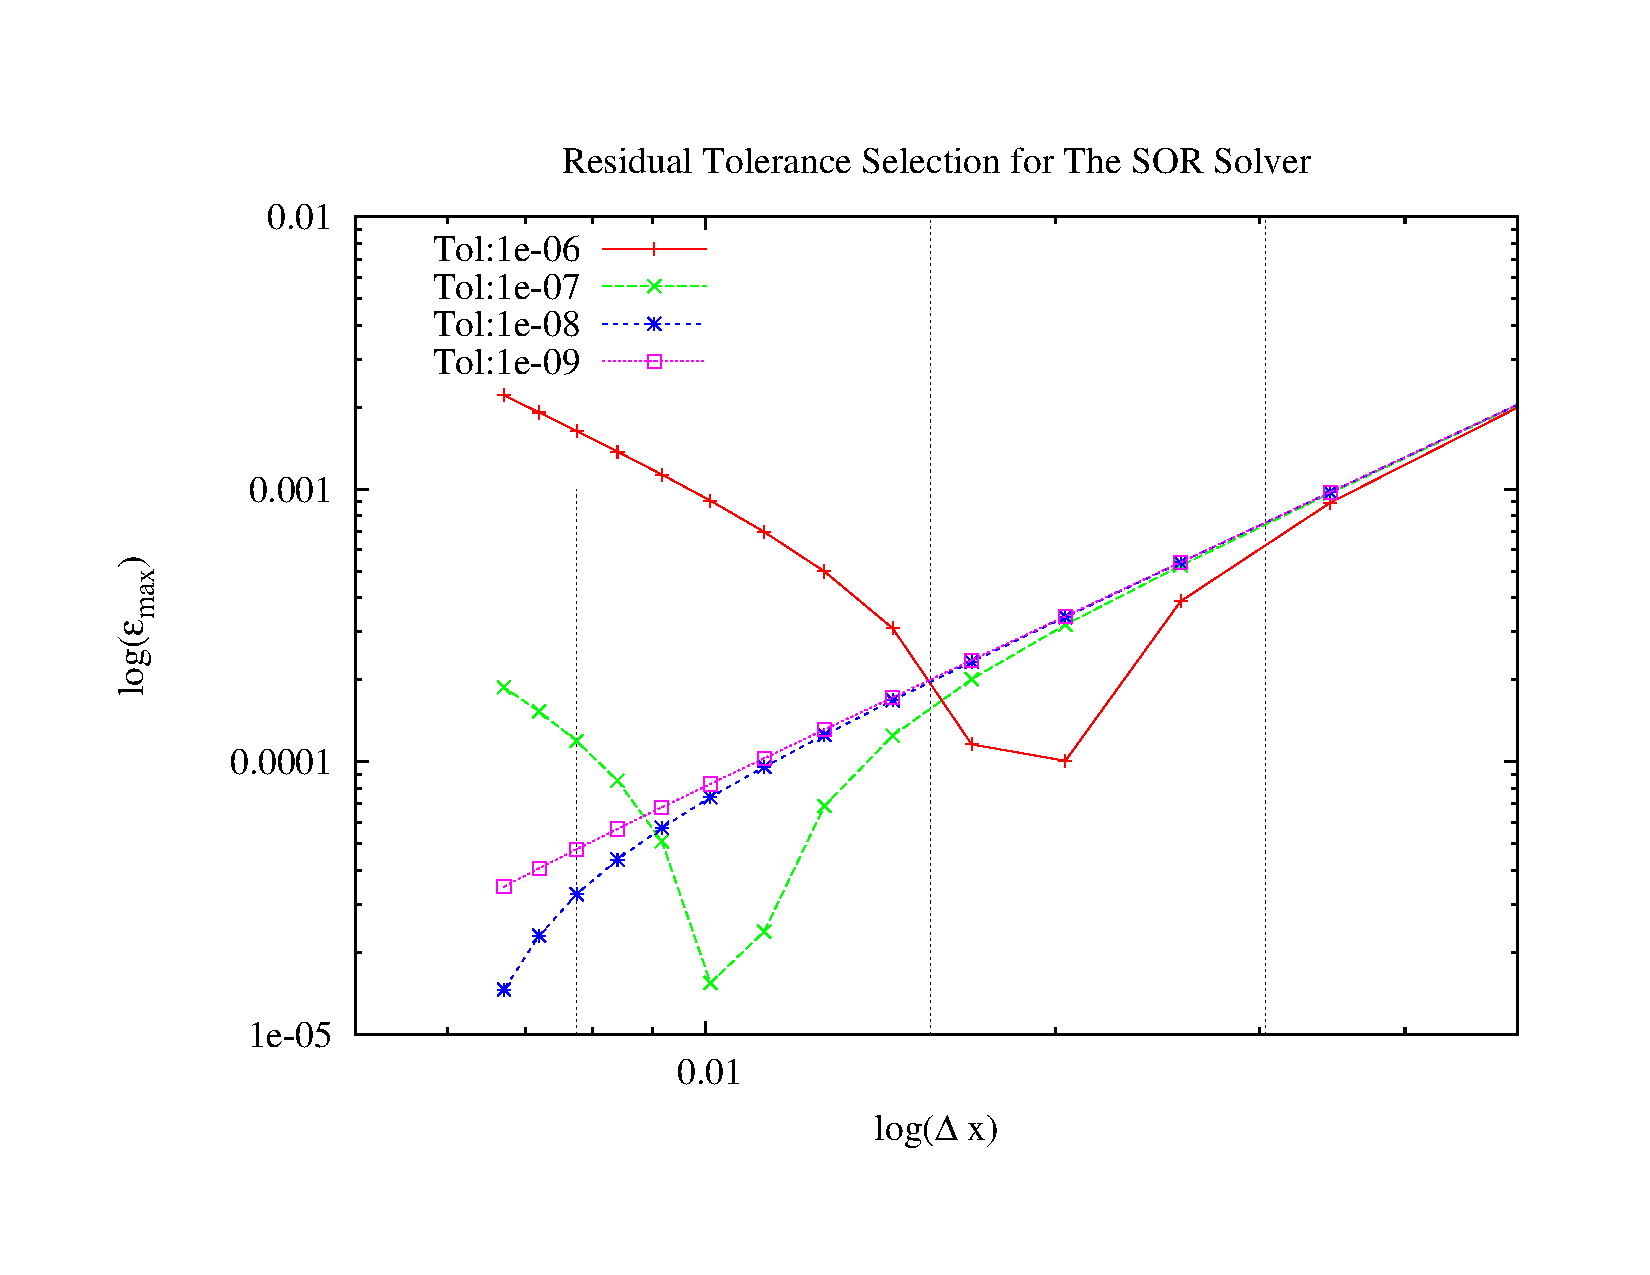
\includegraphics[width=0.9\textwidth]{plots/rts}
\caption{Maximum numerical error as a function of grid spacing, for different residual tolerances, plotted on a log-log scale, for the SOR Solver.}
\label{fig:rts}
\end{figure}

\begin{figure}[h!]
\center
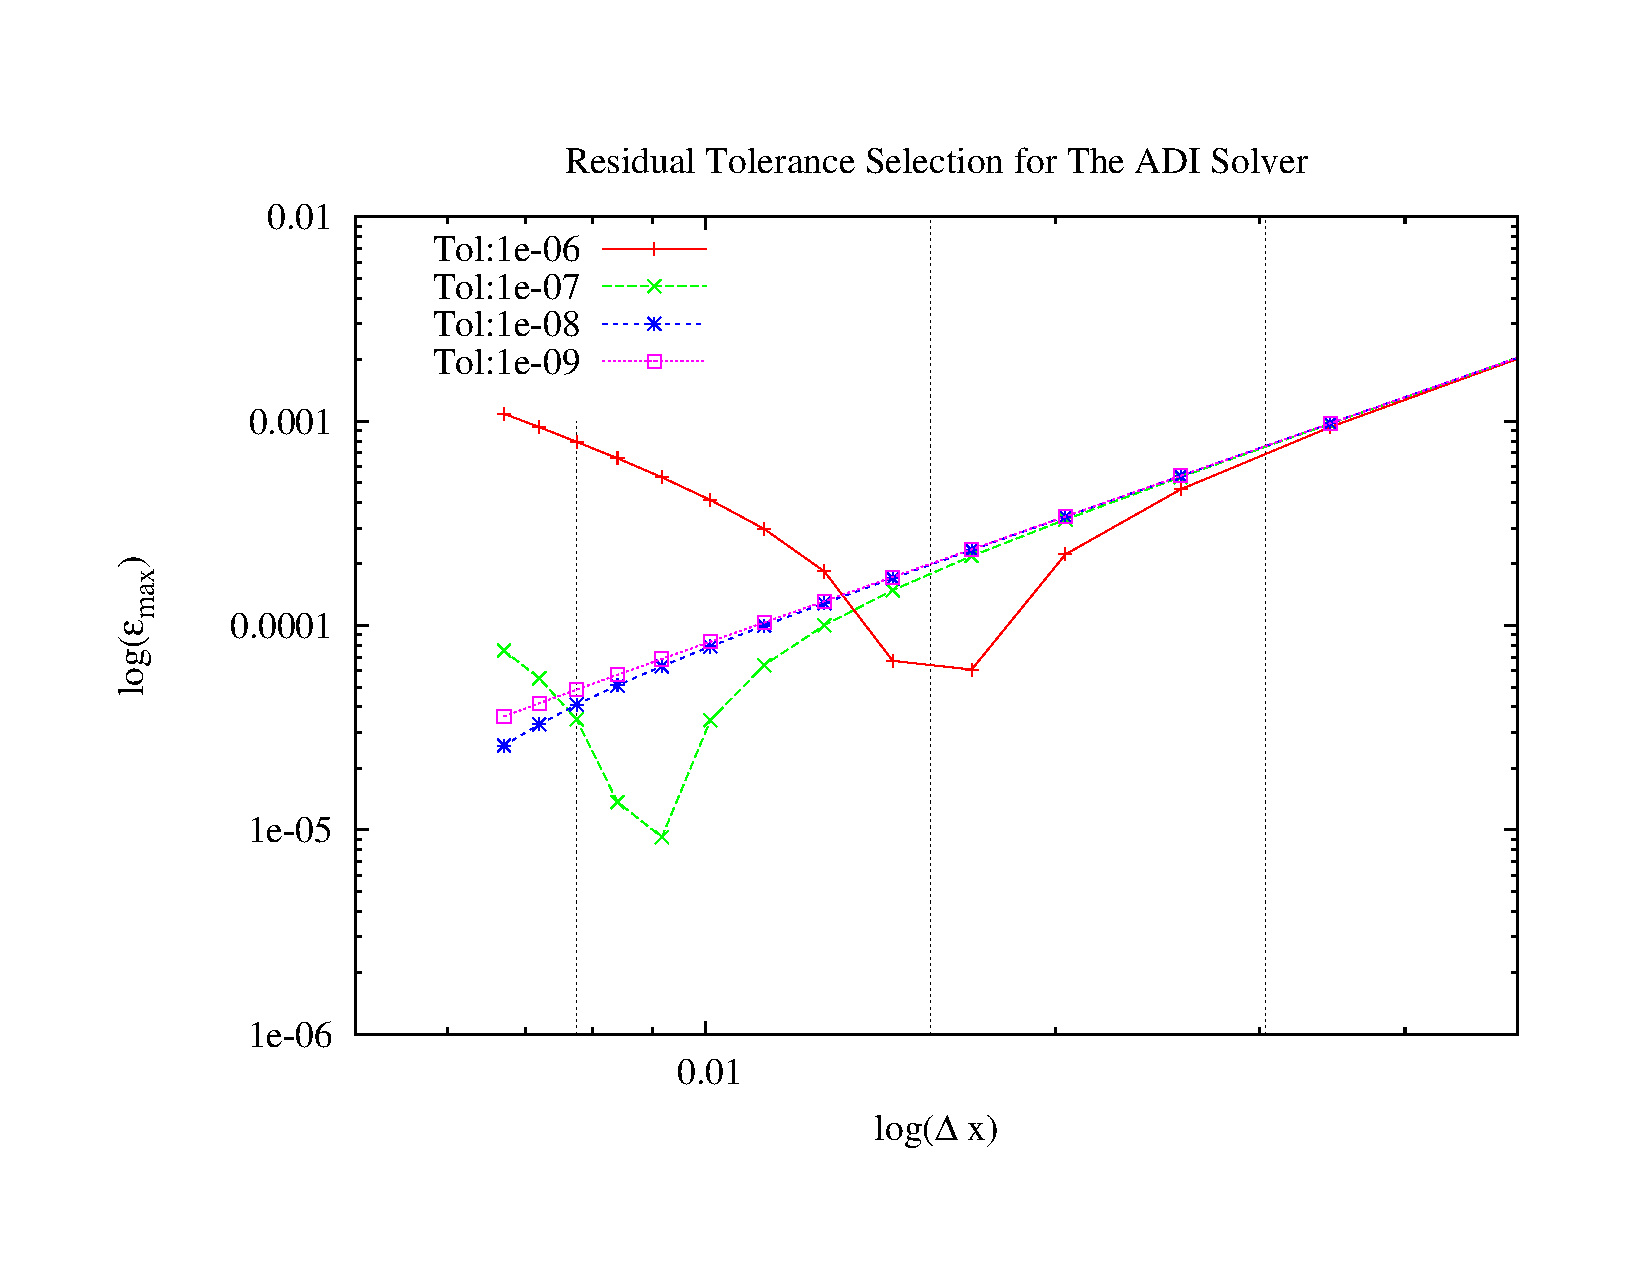
\includegraphics[width=0.9\textwidth]{plots/rta}
\caption{Maximum numerical error as a function of grid spacing, for different residual tolerances, plotted on a log-log scale, for the ADI Solver.}
\label{fig:rta}
\end{figure}


From Figures \ref{fig:rts} and \ref{fig:rta}, the deviation from the linear slope of 2 indicates that the error owing from the residuals is non negligible.  The tolerances were selected such that they were as large as possible, while still maintaining a linear slope, as they crossed the corresponding grid's vertical line, from right to left.  The selected tolerance for each grid is the same for both the SOR and ADI Solvers, and are summarized in Table \ref{tab:rt}.


\begin{table}
\center
\caption{Optimal Residual Tolerance}
\label{tab:rt}

\begin{tabular}{l r}
\hline
Grid Size & Optimal Tolerance \\
\hline 
33x33   & $10^{-7}$  \\
65x65   & $10^{-8}$  \\
129x129 & $10^{-9}$  \\
\hline  
\end{tabular}
\end{table}



	\subsection{Selection of Relaxation Factor for SOR Solver}
	\label{sec:rf_sor}

To pick an optimal relaxation factor $\omega$ for the SOR solver, the parameter was varied from 0.5 to 1.99, in increments of 0.01, and the number of iterations required to solve the Poisson equation was recorded and plotted in Figure \ref{fig:rfs}. The Relaxation Factor yielding the minimum iterations was selected as optimal. For each new value of $\omega$, the same initial conditions for $\psi$ were re-initialized, and the right hand side was kept constant.  The optimal relaxation factors are summarized in Table \ref{tab:rfs}.


\begin{figure}[h!]
\center
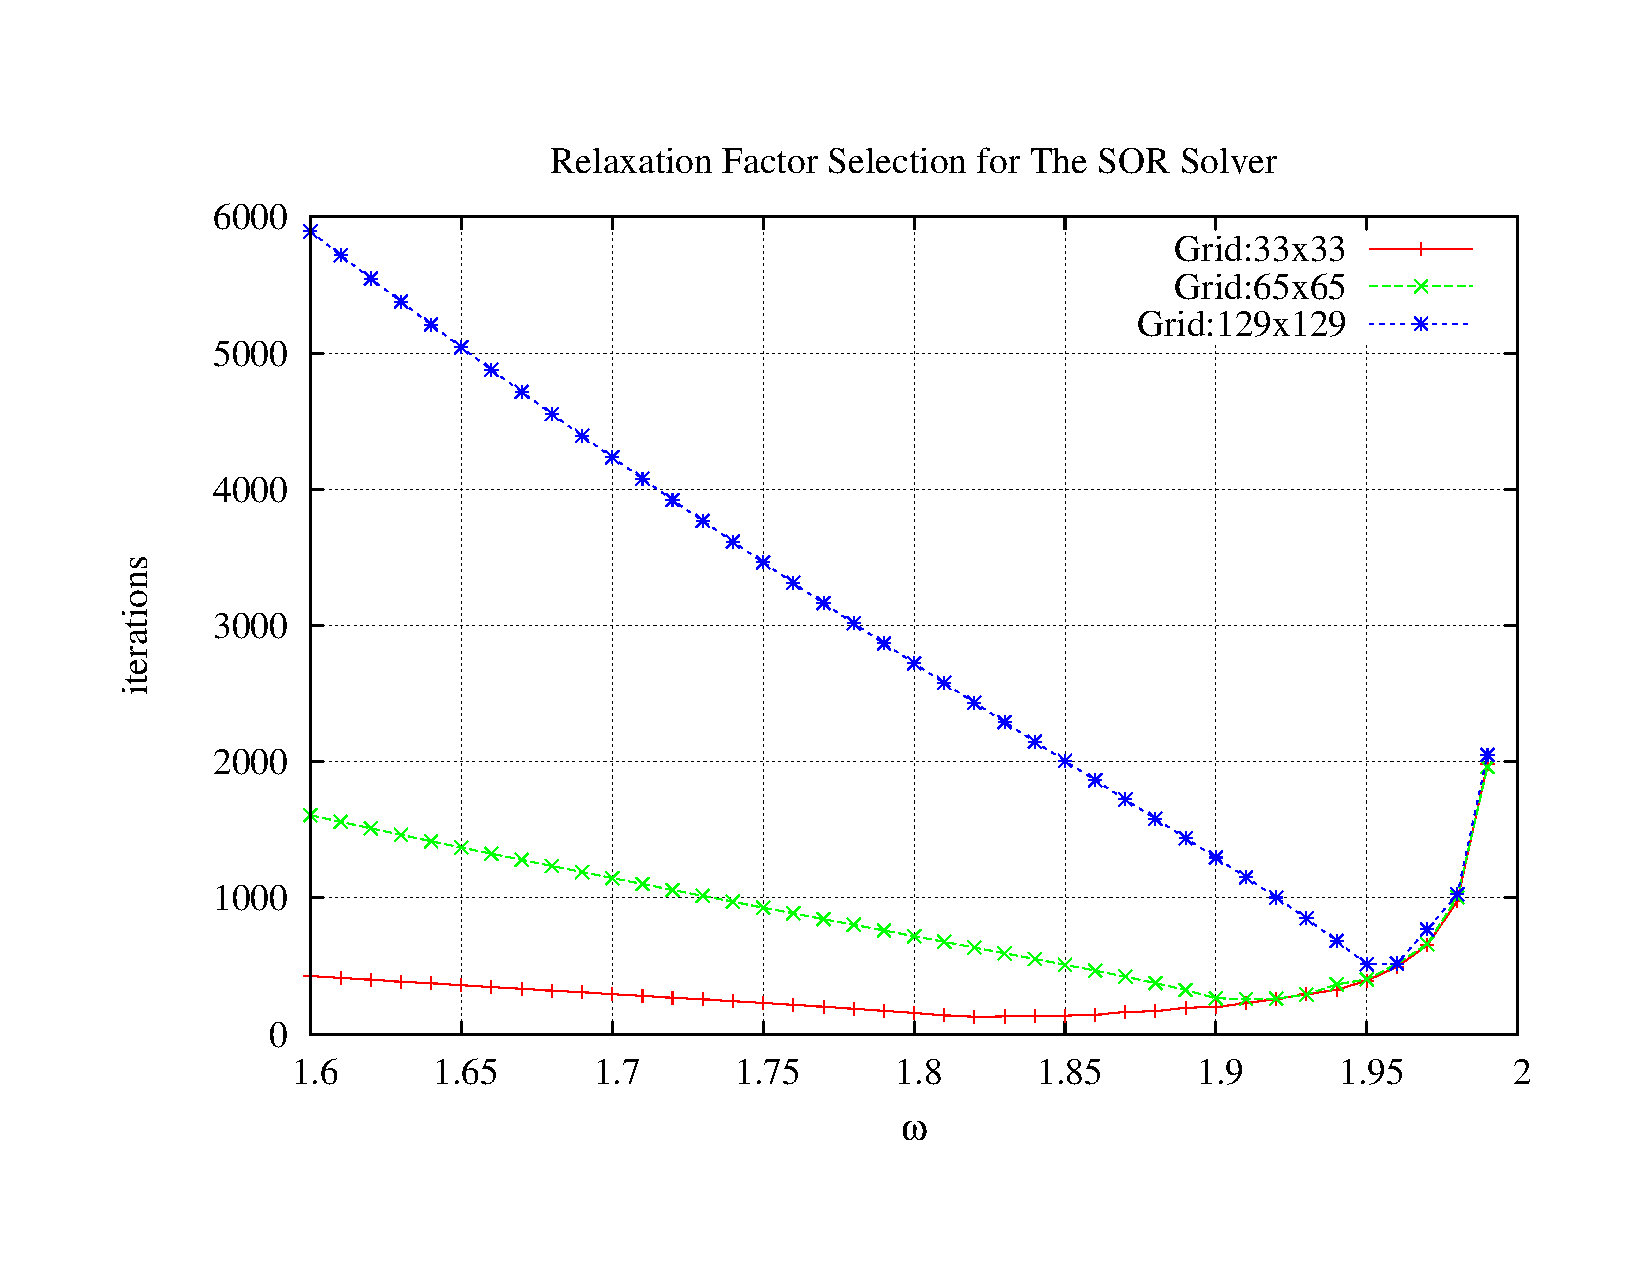
\includegraphics[width=0.9\textwidth]{plots/rfs}
\caption{Number of iterations as a function of The Relaxation Factor for The SOR Solver}
\label{fig:rfs}
\end{figure}


\begin{table}
\center
\caption{Optimal Relaxation Factor $\omega$}
\label{tab:rfs}

\begin{tabular}{l c c r}
\hline
Grid Size & Tolerance & Min. Iterations & $\omega$  \\
\hline
\hline 
33x33   & $10^{-7}$ & 129 & 1.82 \\
65x65   & $10^{-8}$ & 258 & 1.91 \\
129x129 & $10^{-9}$ & 513 & 1.95 \\
\hline  
\end{tabular}
\end{table}



	\subsection{Comparison of SOR and ADI Run Time}
	\label{sec:sor_vs_adi}

The SOR method was many times faster than the ADI method.  Something was not right with the ADI method, but unfortunately the bug was not discovered in time.  The results from the run time test are displayed in Table \ref{tab:sor_vs_adi}, but because of the falsely slow results of the ADI method, nothing can be concluded from this data.


\begin{table}
\center
\caption{Comparison of SOR and ADI Run Times}
\label{tab:sor_vs_adi}

\begin{tabular}{l c c c r}
\hline
Grid & Reynolds & time steps & ADI Runtime & SOR Runtime \\
\hline 
\hline 
$33x33$   & 100 & 161 & 0m1.400   & 0m3.298 \\
$65x65$   & 100 & 161 & 22.173s   & 0m3.298 \\
$129x129$ & 100 & 65  & 2m58.250s & 9.863s  \\
\hline  
\end{tabular}
\end{table}


\section{Model Validation}
\label{sec:mod_vald}



	\subsection{Comparing Steady State Solution with Literature}
	\label{sec:lit_comp}
The results from the simulation were compared with similar computational work done by Ghia Et. Al.  Both studies solve the stream vorticity equation on a uniform $129x129$ grid with second order accurate, finite difference schemes.  Both studies also use second order accurate, centered schemes For the second order derivatives.  For the convective terms in the vorticity equation, Ghia Et. Al. uses a first order, upwind scheme, and a corrective term at the end to provide second order accuracy.  Both studies employ the same physical boundary conditions, but the schemes used to employ them differ slightly, though both are second order accurate \cite{Ghia1982}.

The x component velocity, along the domains vertical center line, and the y component velocity, along the domains horizontal center line are compared with with Ghia Et. Al., for Reynolds Number of 100 and 1000, in Figures \ref{fig:lit_u_100} and \ref{fig:grs_v_1000}.

For the 100 Reynolds Number case, the velocity profiles from the two studies match up quite closely.  In Figure \ref{fig:lit_u_100}, the u-velocity along the vertical center-line shows a slight discrepancy near the top surface though.  At this point, very high velocity gradients are also observed.  The differences in discretization schemes implemented at the boundaries may be more pronounced because of these high gradients, and could be causing these differences. Furthermore, the difference is more noticeable for the higher Reynolds Number case in Figure \ref{fig:lit_u_1000}, where the gradients are also noticeably higher.  Another observation from Figures \ref{fig:lit_u_100} to \ref{fig:lit_v_1000} is that there are noticeable differences between the two curves in places with high curvature.  These differences may be owing to truncation errors, where higher order derivatives become more significant.


\begin{figure}[h!]
\center
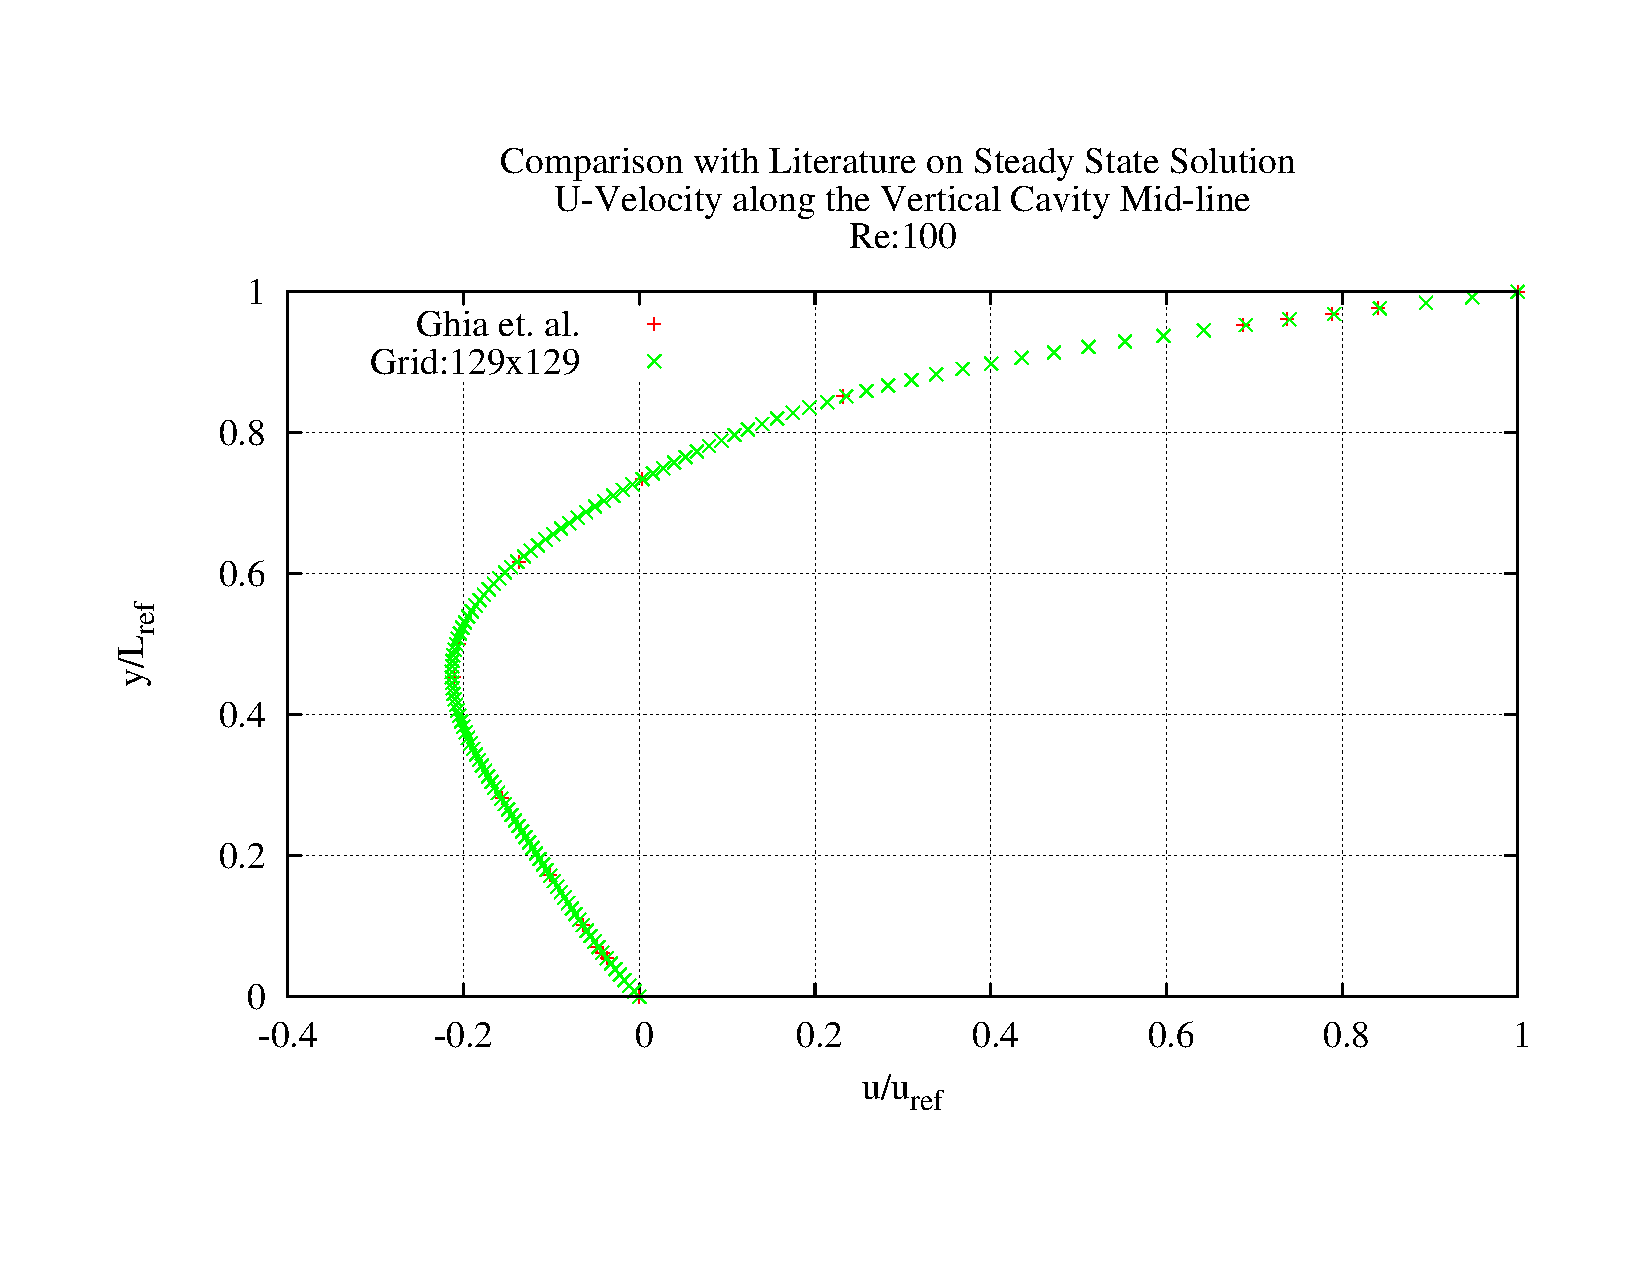
\includegraphics[width=0.9\textwidth]{plots/lit_u_100}
\caption{Steady state u-velocity as a function of y, along the vertical cavity mid-line, at Re:100, for comparison with literature.}
\label{fig:lit_u_100}

\center
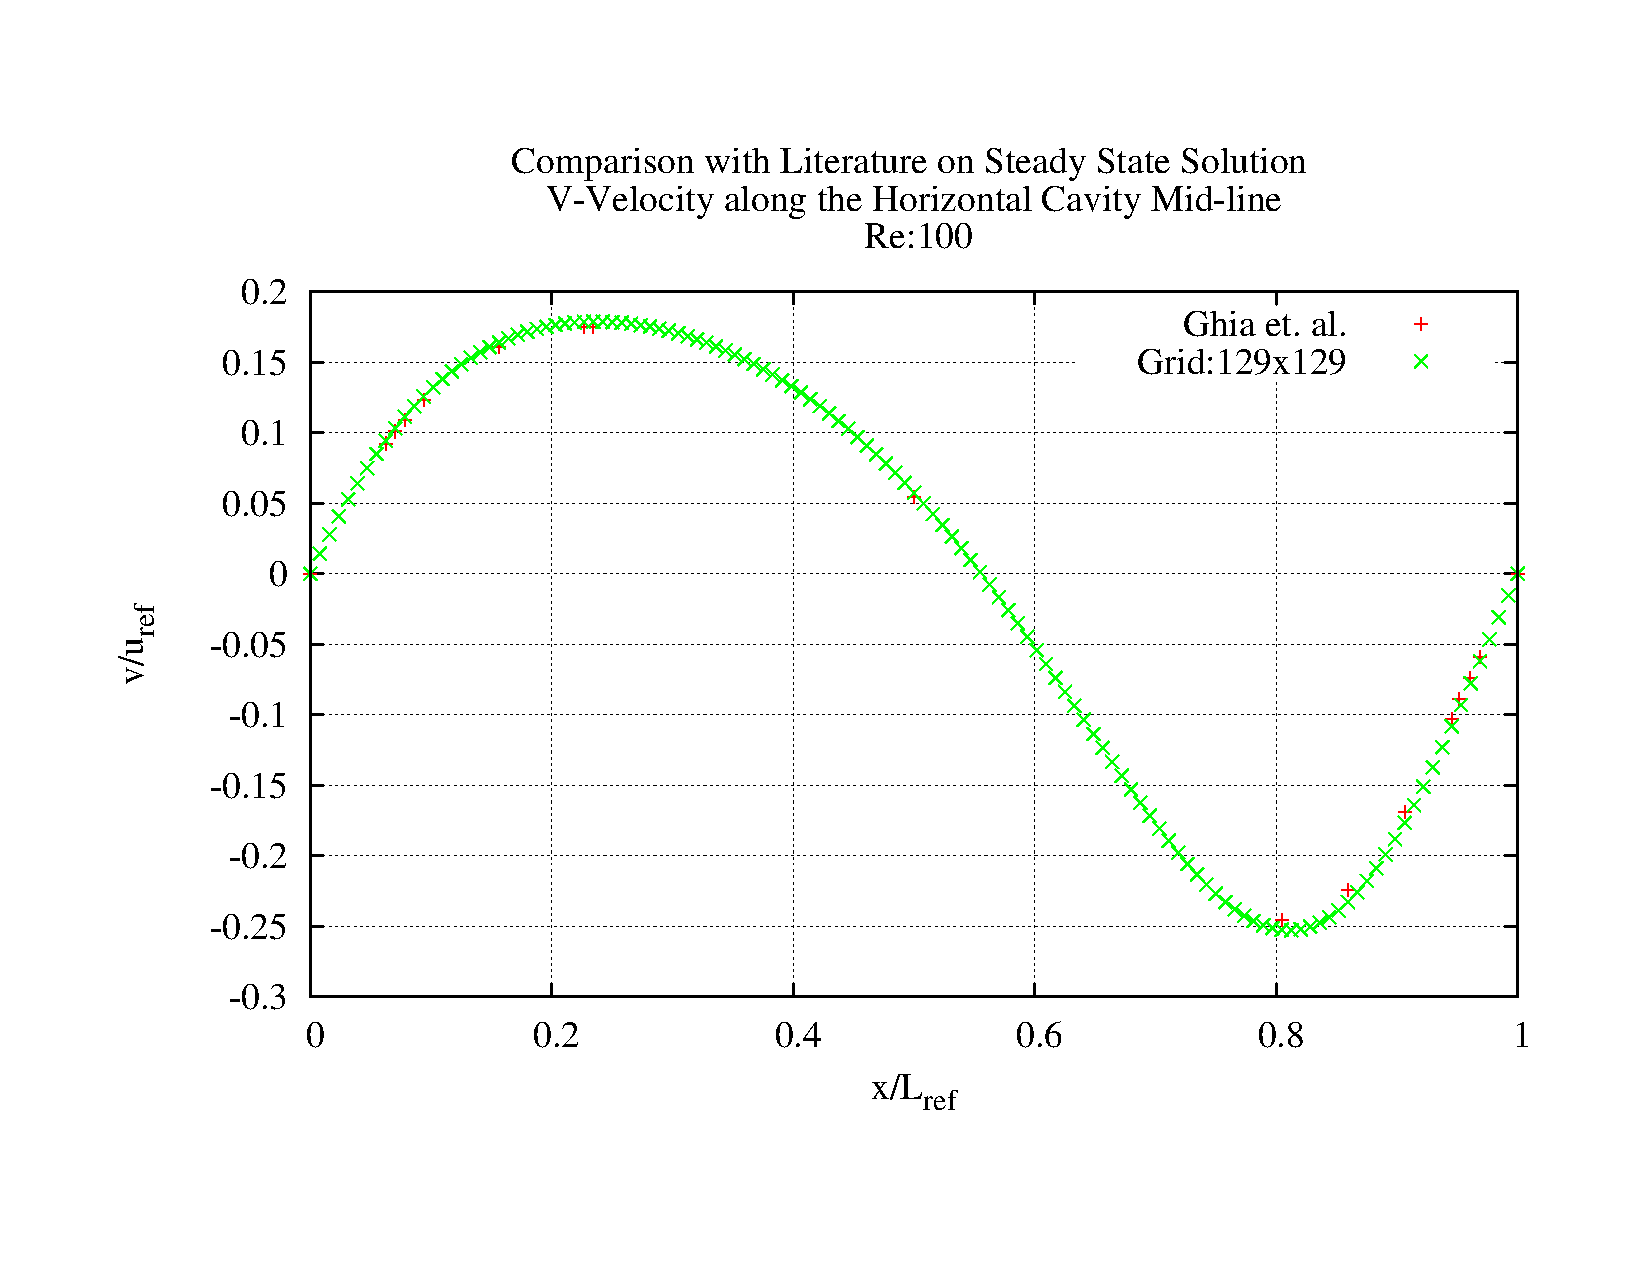
\includegraphics[width=0.9\textwidth]{plots/lit_v_100}
\caption{Steady state v-velocity as a function of x, along the horizontal cavity mid-line, at Re:100, for comparison with literature.}
\label{fig:lit_v_100}
\end{figure}


\begin{figure}[h!]
\center
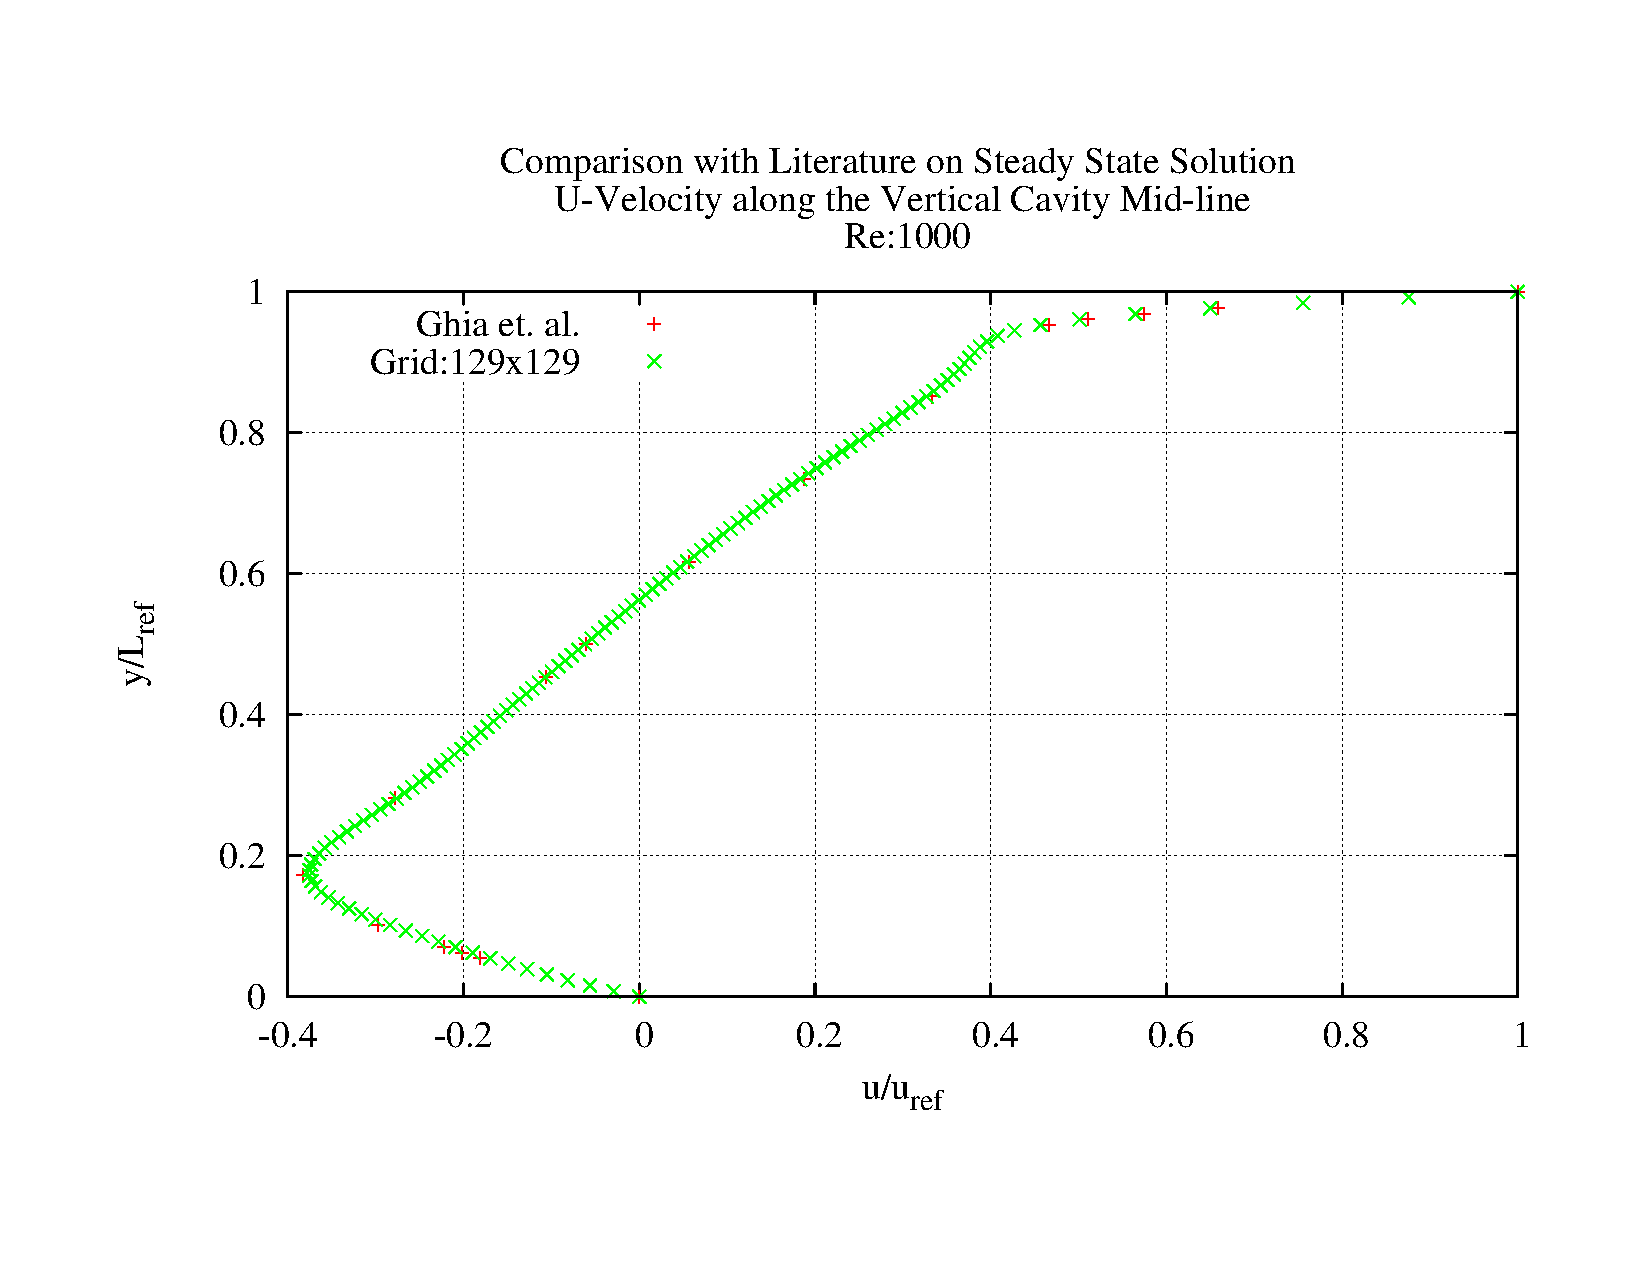
\includegraphics[width=0.9\textwidth]{plots/lit_u_1000}
\caption{Steady state u-velocity as a function of y, along the vertical cavity mid-line, at Re:1000 for comparison with literature}
\label{fig:lit_u_1000}

\center
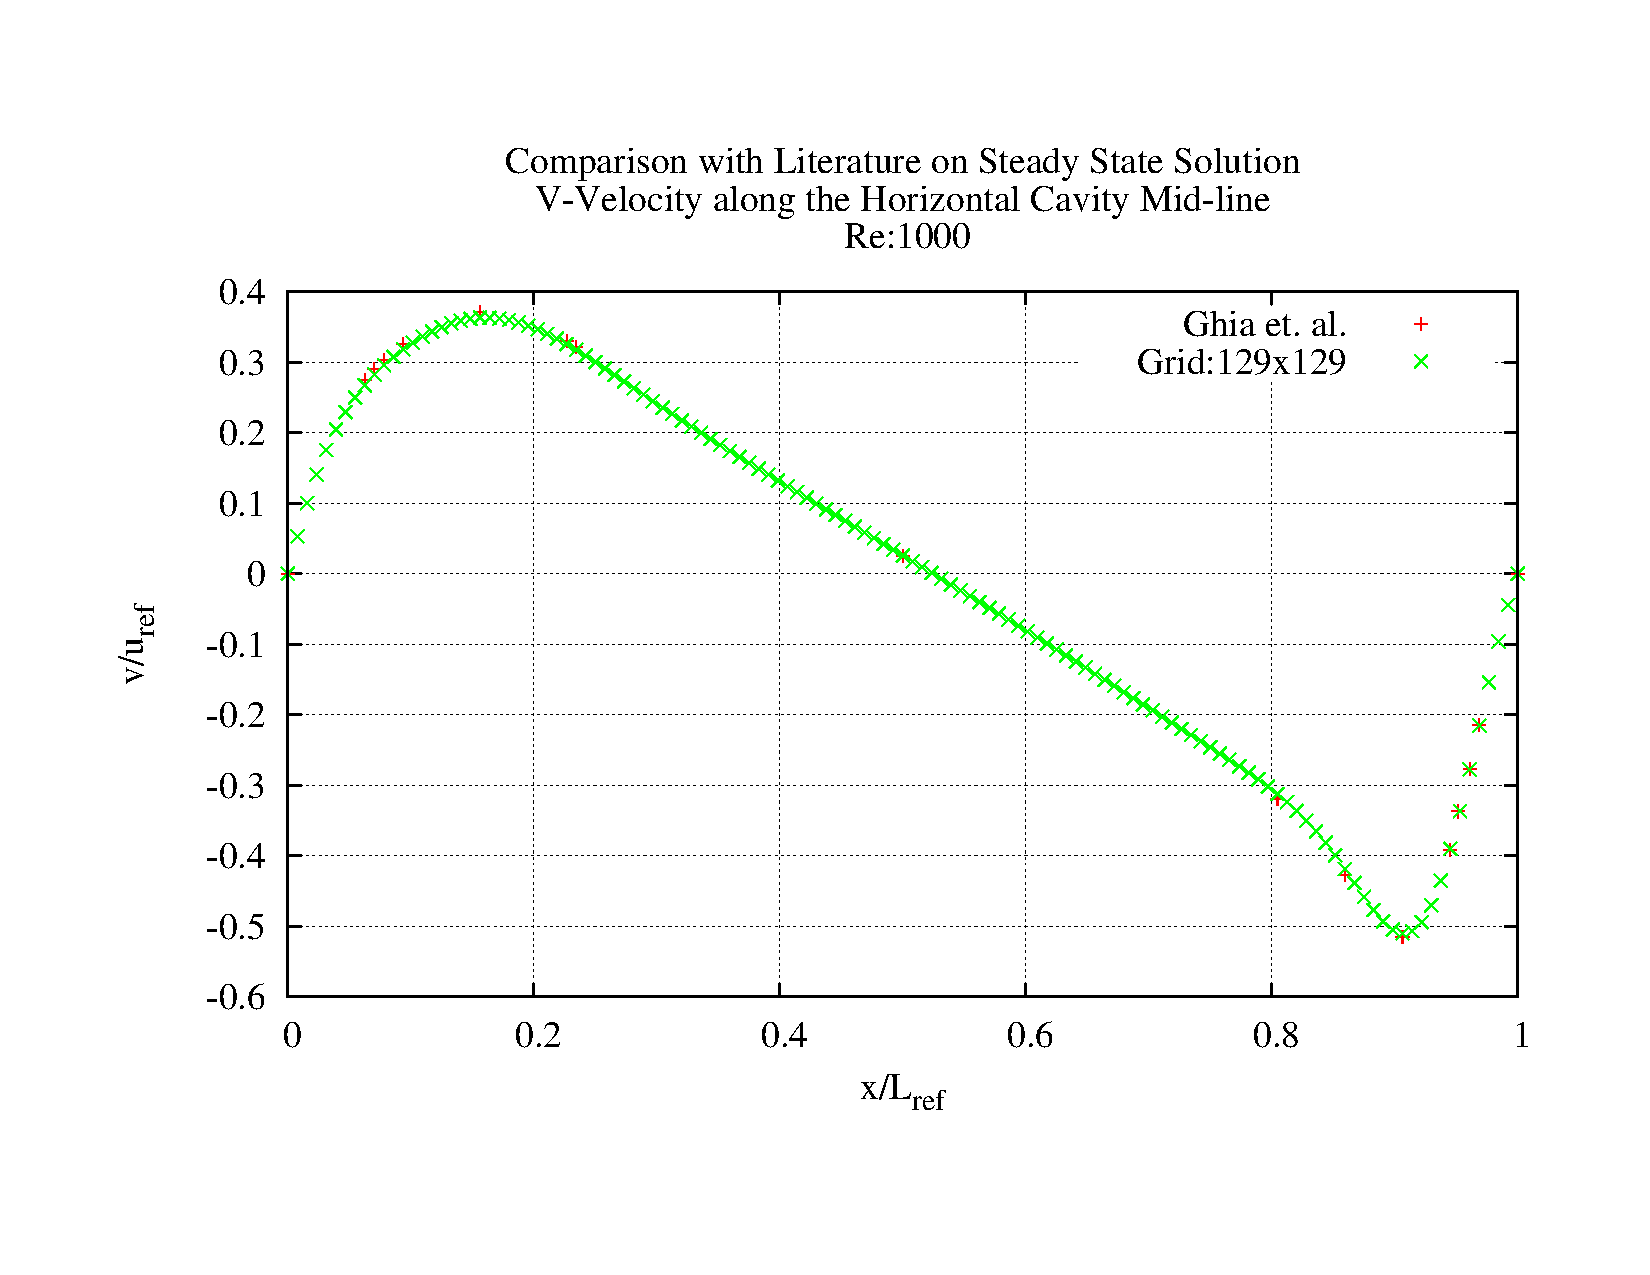
\includegraphics[width=0.9\textwidth]{plots/lit_v_1000}
\caption{Steady state v-velocity as a function of x, along the horizontal cavity mid-line, at Re:1000 for comparison with literature.}
\label{fig:lit_v_1000}
\end{figure}


	\subsection{Effect of Grid Refinement on Steady State Solution}

Having validated the fine grid solution with literature, grid spacing and its affects on the steady state solution was examined.  Simulations were run on $33x33$ and $65x65$ grids, and  were compared to simulations on the fine grid.  The u-velocity along the vertical centerline, and v-velocity along the horizontal centerline is plotted for the 3 grids in Figures \ref{fig:grs_u_100} to \ref{fig:grs_v_1000}.

\begin{figure}[h!]
\center
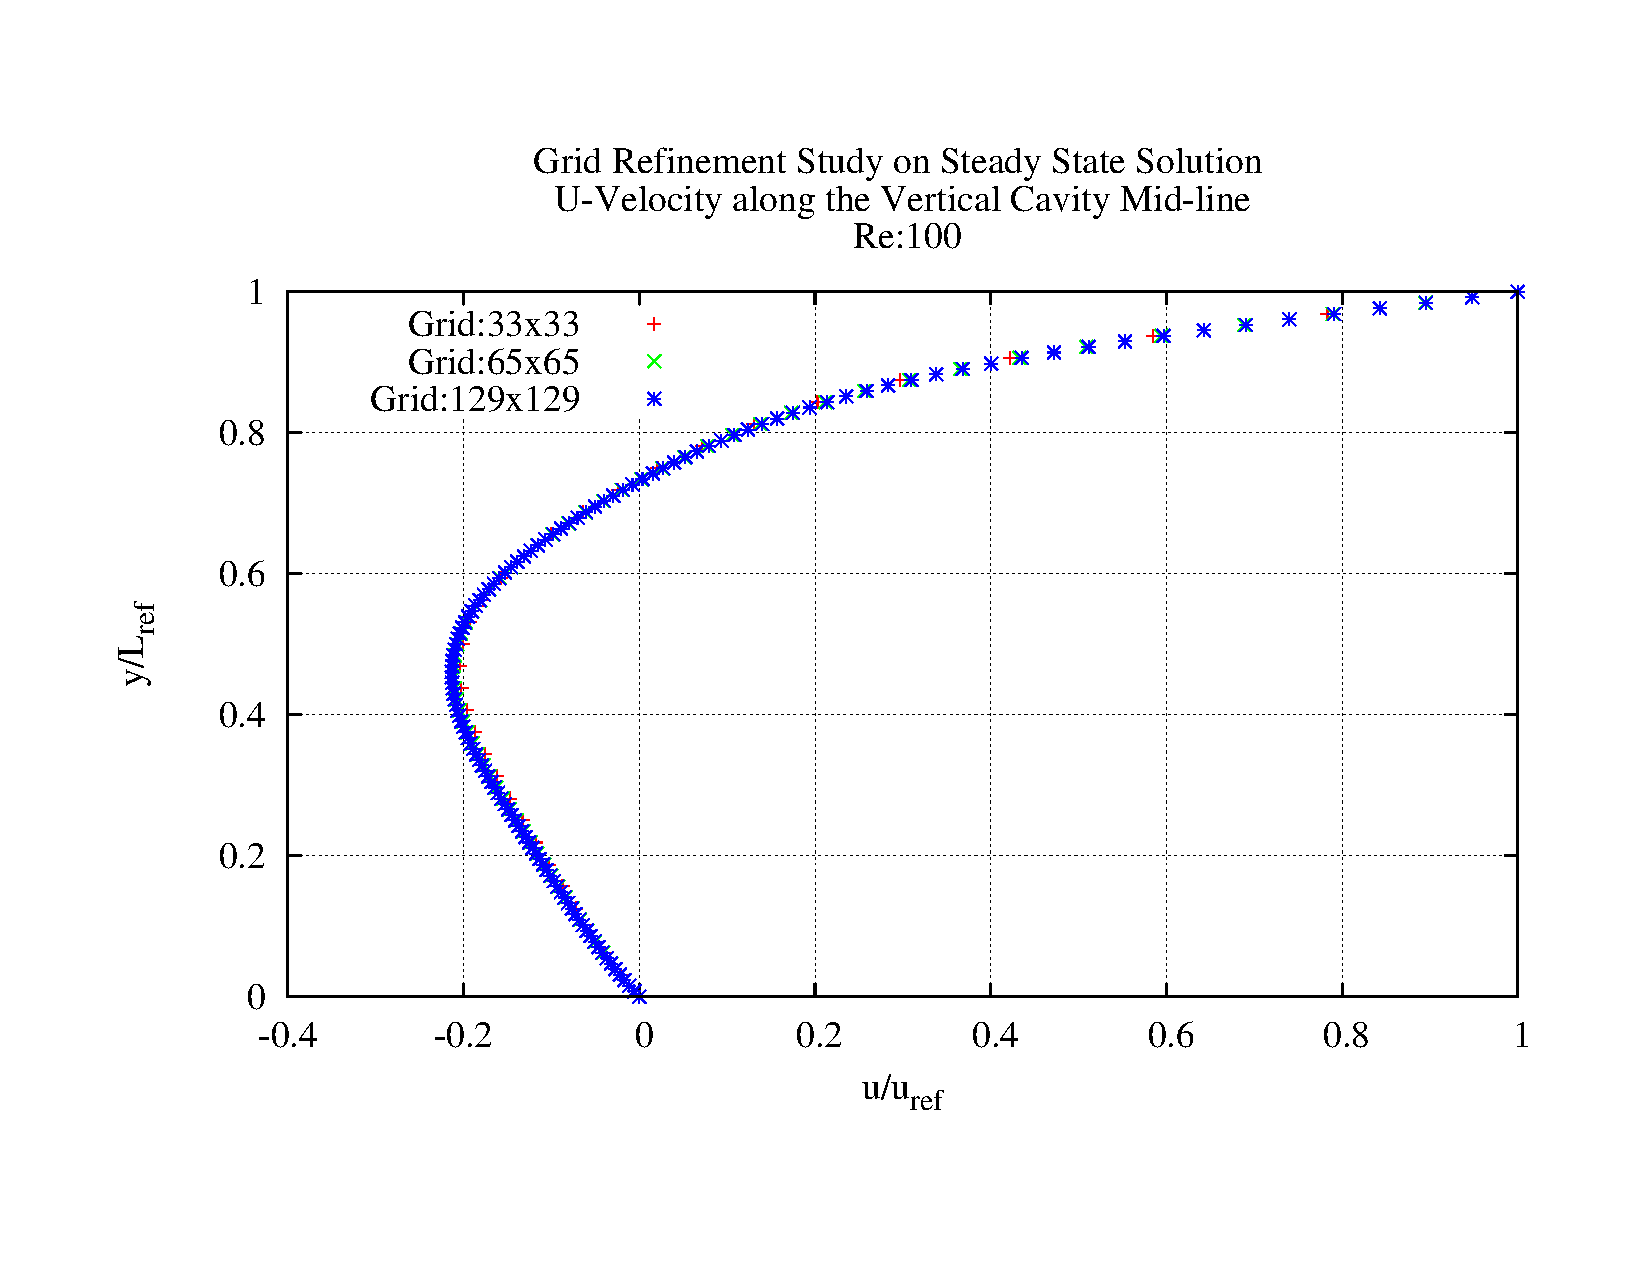
\includegraphics[width=0.9\textwidth]{plots/grs_u_100}
\caption{Steady state u-velocity as a function of y, along the vertical cavity mid-line, for 3 different grid sizes, at Re:100.}
\label{fig:grs_u_100}

\center
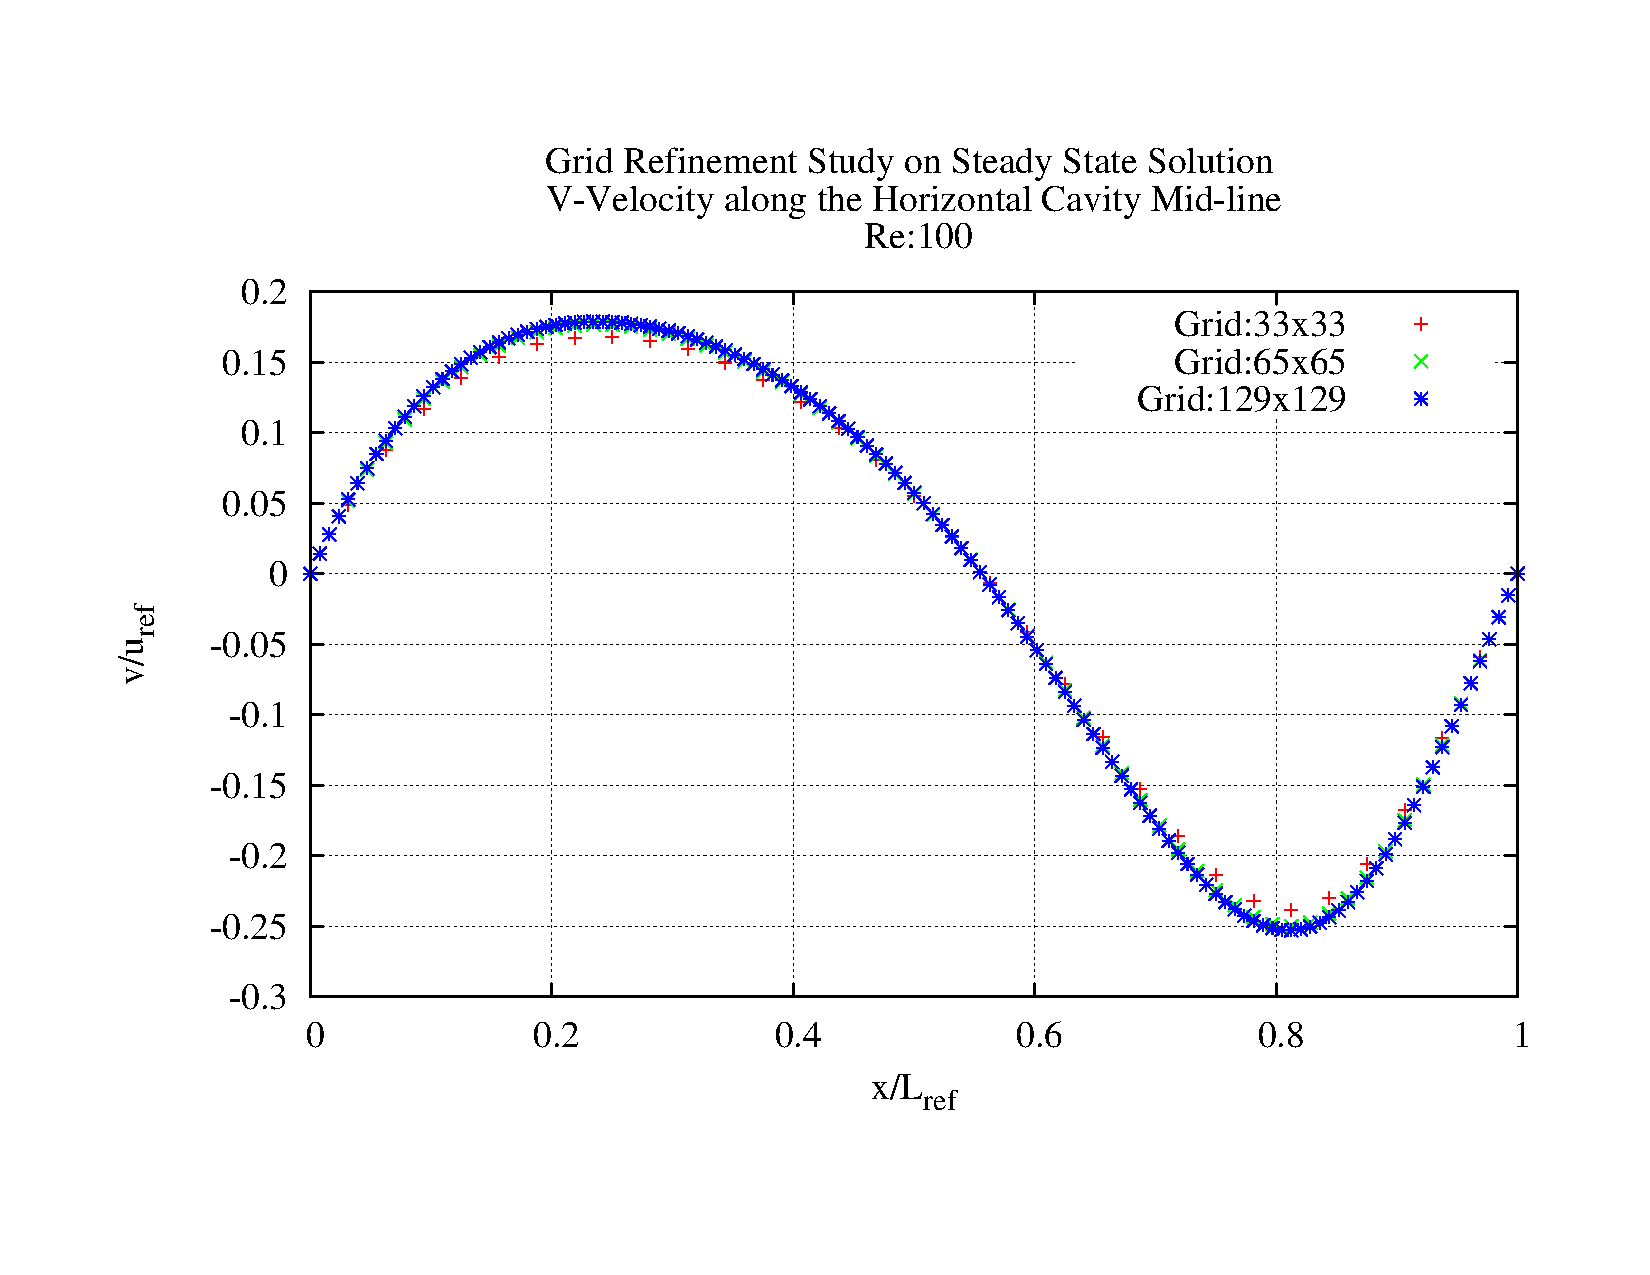
\includegraphics[width=0.9\textwidth]{plots/grs_v_100}
\caption{Steady state v-velocity as a function of x, along the horizontal cavity mid-line, for 3 different grid sizes, at Re:100.}
\label{fig:grs_v_100}
\end{figure}

\begin{figure}[h!]
\center
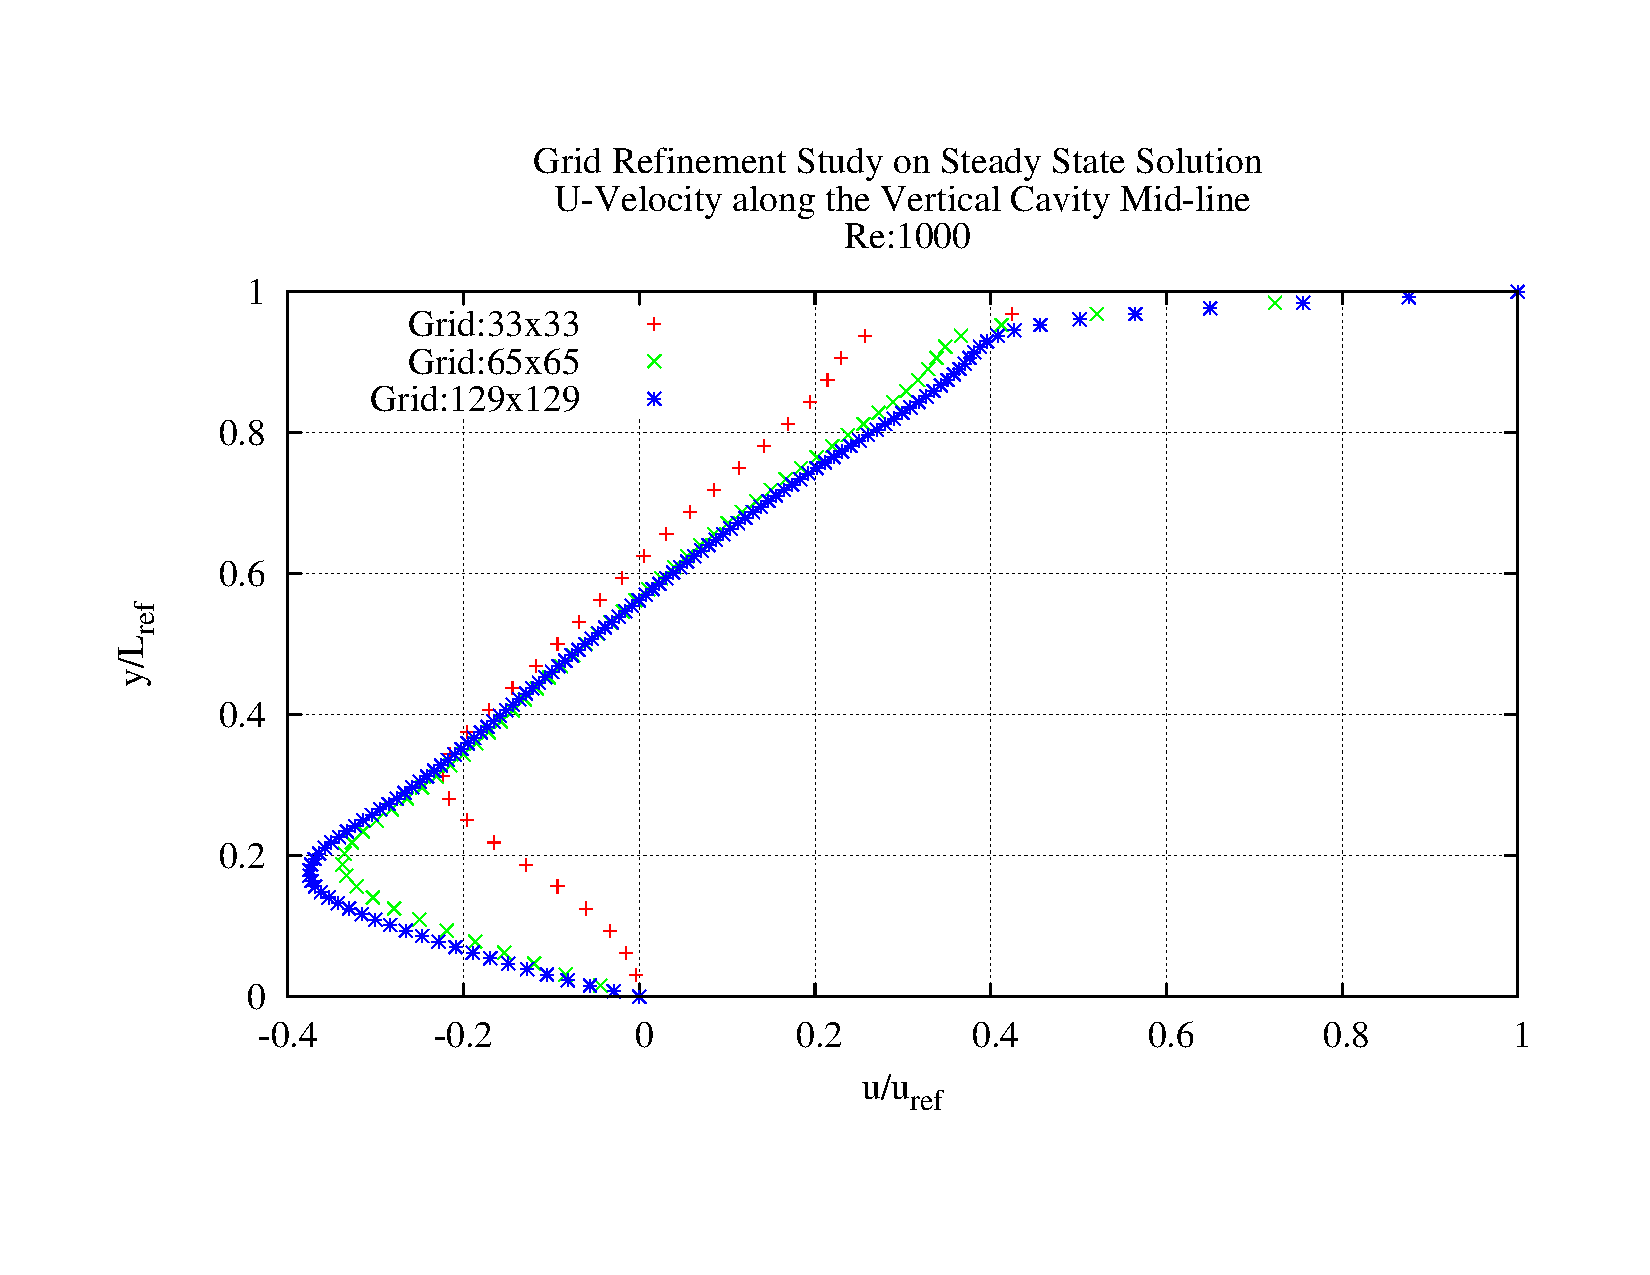
\includegraphics[width=0.9\textwidth]{plots/grs_u_1000}
\caption{Steady state u-velocity as a function of y, along the vertical cavity mid-line, for 3 different grid sizes, at Re:1000.}
\label{fig:grs_u_1000}

\center
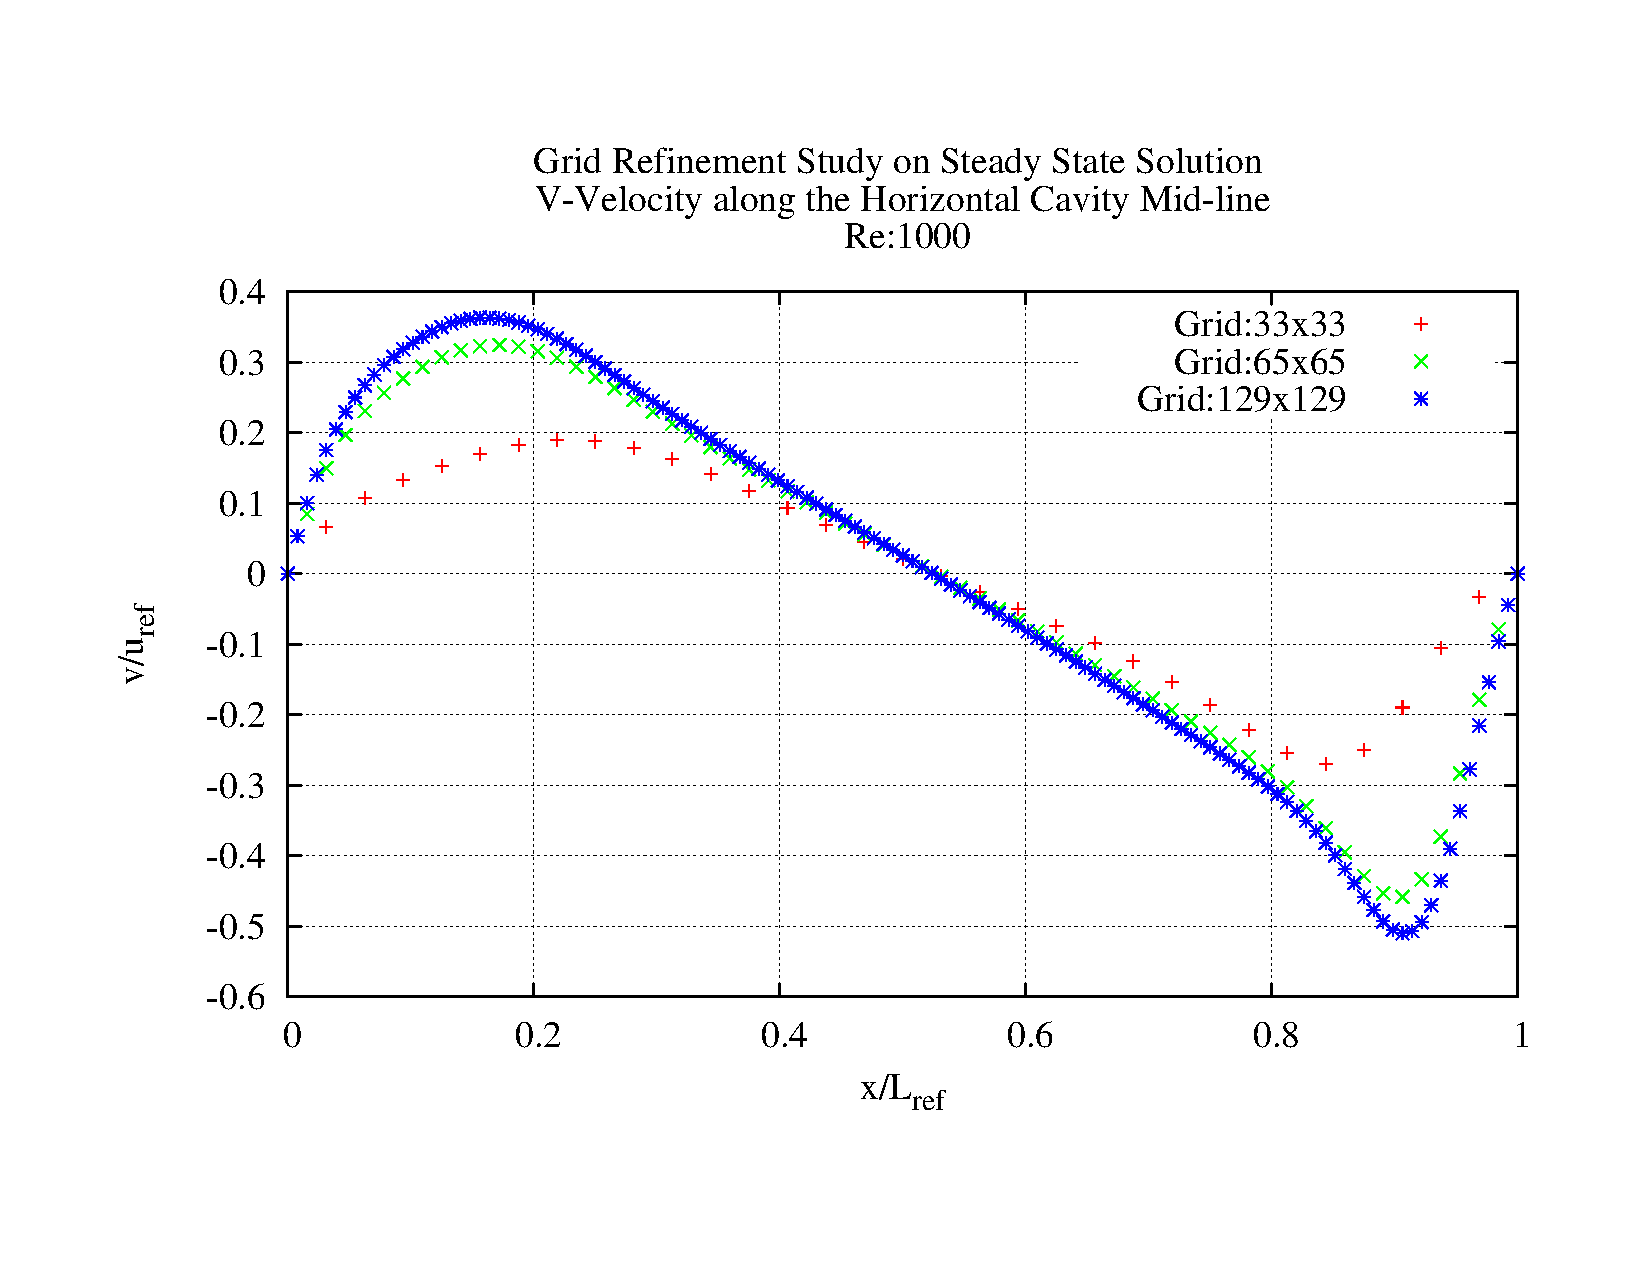
\includegraphics[width=0.9\textwidth]{plots/grs_v_1000}
\caption{Steady state v-velocity as a function of x, along the vertical cavity mid-line, for 3 different grid sizes, at Re:1000.}
\label{fig:grs_v_1000}
\end{figure}

At the lower Reynolds Number, Both the medium and the coarse grid are very close to the fine grid solution.  In areas where the velocity has high curvature, the coarse grid deviates slightly off from the other two grid's velocity profile.  

For the high Reynolds Number, the medium grid deviates slightly off the fine grid solution.  The coarse grid has a significantly different profile in areas with steep gradients, near the boundaries.  The error induced by steep gradients at the boundaries propagates inwards, and as a results, the coarse grid is never really accurate.  Close to the center of the domain, where the profiles are flat, the coarse grid has a similar shape to the other grids, but error from the boundaries causes the solution to be drastically different.  Since the truncation error is proportional to $\Delta x^2$, for the numerical schemes implemented, this is not a surprising result.  The leading truncation error term is 16 times larger than that of the fine grid. As a result, truncation errors, which become significant in areas with changes in curvature, are 16 times higher in the coarse grid, then the fine grid.



\chapter{Conclusion}


The discretization schemes used in this study were shown to be second order accurate.  They yielded almost identical results to a similar study by Ghia Et. Al., but slight differences were evident near the walls.  It's believed that differences in boundary condition implementation was a major contributing factor to these discrepancies. 

The ADI method was used to speed up the computation.  Unfortunately, there was a bug in the method, and in the end, the ADI method was far slower than SOR.  This bug did not affect the ADI methods final solution, but it drastically increased the time required to converge to a solution.  It is suspected that the bug lies somewhere in the optimal time step selection, for fast convergence, or in the method for solving tri-diagonal systems.  Further de-bugging is required before any concrete conclusions can be drawn on why the ADI method is so slow to converge.

Some instabilities were observed with a CFL number greater than 0.5.  A stability analysis should be performed for the FTCS scheme implemented to determine if this observation is expected.  After completing a stability analysis, some criteria should be provided for CFL Number selection.  Currently, the largest CFL number yielding a stable solutions is 0.2, and one should be cautious when running the program with larger CFL Numbers.

The program is structured such that it can be adapted to solve problems on a variety of grids.  The class constructors, numerical schemes, and VTK data writer must be adapted accordingly.  Future work includes solving these equations on a variety of domains involving more complicated geometry.  Additionally, the 3D Navier Stokes equations could be implemented.  Additionally, the VTK package should be included as a runtime argument.  Currently, the program is duplicated to run without VTK, but that version will not stay current with any future modifications.

%% Some commands used in this file
\newcommand{\package}{\emph}

\chapter{Introduction}

This is version \verb-v1.4- of the template.

We assume that you found this template on our institute's website, so
we do not repeat everything stated there.  Consult the website again
for pointers to further reading about \LaTeX{}.  This chapter only
gives a brief overview of the files you are looking at.

\section{Features}
\label{sec:features}

The rest of this document shows off a few features of the template
files.  Look at the source code to see which macros we used!

The template is divided into \TeX{} files as follows:
\begin{enumerate}
\item \texttt{thesis.tex} is the main file.
\item \texttt{extrapackages.tex} holds extra package includes.
\item \texttt{layoutsetup.tex} defines the style used in this document.
\item \texttt{theoremsetup.tex} declares the theorem-like environments.
\item \texttt{macrosetup.tex} defines extra macros that you may find
  useful.
\item \texttt{introduction.tex} contains this text.
\item \texttt{sections.tex} is a quick demo of each sectioning level
  available.
\item \texttt{refs.bib} is an example bibliography file.  You can use
  Bib\TeX{} to quote references.  For example, read
  \cite{bringhurst1996ets} if you can get a hold of it.
\end{enumerate}


\subsection{Extra package includes}

The file \texttt{extrapackages.tex} lists some packages that usually
come in handy.  Simply have a look at the source code.  We have
added the following comments based on our experiences:
\begin{description}
\item[REC] This package is recommended.
\item[OPT] This package is optional.  It usually solves a specific
  problem in a clever way.
\item[ADV] This package is for the advanced user, but solves a problem
  frequent enough that we mention it. Consult the package's
  documentation.
\end{description}

As a small example, here is a reference to the Section \emph{Features}
typeset with the recommended \package{varioref} package:
\begin{quote}
  See Section~\vref{sec:features}.
\end{quote}


\subsection{Layout setup}

This defines the overall look of the document -- for example, it
changes the chapter and section heading appearance.  We consider this
a `do not touch' area.  Take a look at the excellent \emph{Memoir}
documentation before changing it.

In fact, take a look at the excellent \emph{Memoir} documentation,
full stop.


\subsection{Theorem setup}

This file defines a bunch of theorem-like environments.

\begin{theorem}
  An example theorem.
\end{theorem}

\begin{proof}
  Proof text goes here.
\end{proof}

Note that the q.e.d.\ symbol moves to the correct place automatically
if you end the proof with an \texttt{enumerate} or
\texttt{displaymath}.  You do not need to use \verb-\qedhere- as with
\package{amsthm}.

\begin{theorem}[Some Famous Guy]
  Another example theorem.
\end{theorem}

\begin{proof}
  This proof
  \begin{enumerate}
  \item ends in an enumerate.
  \end{enumerate}
\end{proof}

\begin{proposition}
  Note that all theorem-like environments are by default numbered on
  the same counter.
\end{proposition}

\begin{proof}
  This proof ends in a display like so:
  \begin{displaymath}
    f(x) = x^2.
  \end{displaymath}
\end{proof}


\subsection{Macro setup}

For now the macro setup only shows how to define some basic macros,
and how to use a neat feature of the \package{mathtools} package:
\begin{displaymath}
  \abs{a}, \quad \abs*{\frac{a}{b}}, \quad \abs[\big]{\frac{a}{b}}.
\end{displaymath}

%\chapter{Writing scientific texts in English}

This chapter was originally a separate document written by Reto
Spöhel.  It is reprinted here so that the template can serve as a
quick guide to thesis writing, and to provide some more example
material to give you a feeling for good typesetting.

% We're going to need an extra theorem-like environment for this
% chapter
\theoremstyle{plain}
\theoremsymbol{}
\newtheorem{Rule}[theorem]{Rule}

\section{Basic writing rules}

The following rules need little further explanation; they are best
understood by looking at the example in the booklet by Knuth et al.,
§2--§3.

\begin{Rule}
  Write texts, not chains of formulas.
\end{Rule}

More specifically, write full sentences that are logically
interconnected by phrases like `Therefore', `However', `On the other
hand', etc.\ where appropriate.

\begin{Rule}
  Displayed formulas should be embedded in your text and punctuated
  with it.
\end{Rule}

In other words, your writing should not be divided into `text parts'
and `formula parts'; instead the formulas should be tied together by
your prose such that there is a natural flow to your writing.

\section{Being nice to the reader}

Try to write your text in such a way that a reader enjoys reading
it. That's of course a lofty goal, but nevertheless one you should
aspire to!

\begin{Rule}
  Be nice to the reader.
\end{Rule}

Give some intuition or easy example for definitions and theorems which
might be hard to digest. Remind the reader of notations you introduced
many pages ago -- chances are he has forgotten them. Illustrate your
writing with diagrams and pictures where this helps the reader. Etc.

\begin{Rule}
  Organize your writing.
\end{Rule}

Think carefully about how you subdivide your thesis into chapters,
sections, and possibly subsections.  Give overviews at the beginning
of your thesis and of each chapter, so the reader knows what to
expect. In proofs, outline the main ideas before going into technical
details. Give the reader the opportunity to `catch up with you' by
summing up your findings periodically.

\emph{Useful phrases:} `So far we have shown that \ldots', `It remains
to show that \ldots', `Recall that we want to prove inequality (7), as
this will allow us to deduce that \ldots', `Thus we can conclude that
\ldots. Next, we would like to find out whether \ldots', etc.

\begin{Rule}
  Don't say the same thing twice without telling the reader that you
  are saying it twice.
\end{Rule}

Repetition of key ideas is important and helpful. However, if you
present the same idea, definition or observation twice (in the same or
different words) without telling the reader, he will be looking for
something new where there is nothing new.

\emph{Useful phrases:} `Recall that [we have seen in Chapter 5 that]
\ldots', `As argued before / in the proof of Lemma 3, \ldots', `As
mentioned in the introduction, \ldots', `In other words, \ldots', etc.

\begin{Rule}
  Don't make statements that you will justify later without telling
  the reader that you will justify them later.
\end{Rule}

This rule also applies when the justification is coming right in the
next sentence!  The reasoning should be clear: if you violate it, the
reader will lose valuable time trying to figure out on his own what
you were going to explain to him anyway.

\emph{Useful phrases:} `Next we argue that \ldots', `As we shall see,
\ldots', `We will see in the next section that \ldots, etc.


\section{A few important grammar rules}

\begin{Rule}
  \label{rule:no-comma-before-that}
  There is (almost) \emph{never} a comma before `that'.
\end{Rule}

It's really that simple. Examples:
\begin{quote}
  We assume that \ldots\\
  \emph{Wir nehmen an, dass \ldots}

  It follows that \ldots\\
  \emph{Daraus folgt, dass \ldots}

  `thrice' is a word that is seldom used.\\
  \emph{`thrice' ist ein Wort, das selten verwendet wird.}
\end{quote}
Exceptions to this rule are rare and usually pretty obvious. For
example, you may end up with a comma before `that' because `i.e.' is
spelled out as `that is':
\begin{quote}
  For \(p(n)=\log n/n\) we have \ldots{} However, if we choose \(p\) a
  little bit higher, that is \(p(n)=(1+\varepsilon)\log n/n\) for some
  \(\varepsilon>0\), we obtain that\ldots
\end{quote}
Or you may get a comma before `that' because there is some additional
information inserted in the middle of your sentence:
\begin{quote}
  Thus we found a number, namely \(n_0\), that satisfies equation (13).
\end{quote}
If the additional information is left out, the sentence has no comma:
\begin{quote}
  Thus we found a number that satisfies equation (13).
\end{quote}
(For `that' as a relative pronoun, see also
Rules~\ref{rule:non-defining-has-comma}
and~\ref{rule:defining-without-comma} below.)

\begin{Rule}
  There is usually no comma before `if'.
\end{Rule}

Example:
\begin{quote}
  A graph is not \(3\)-colorable if it contains a \(4\)-clique.\\
  \emph{Ein Graph ist nicht \(3\)-färbbar, wenn er eine \(4\)-Clique
    enthält.}
\end{quote}
However, if the `if' clause comes first, it is usually separated from
the main clause by a comma:
\begin{quote}
  If a graph contains a \(4\)-clique, it is not \(3\)-colorable .\\
  \emph{Wenn ein Graph eine \(4\)-Clique enthält, ist er nicht
    \(3\)-färbbar.}
\end{quote}

There are more exceptions to these rules than to
Rule~\ref{rule:no-comma-before-that}, which is why we are not
discussing them here. Just keep in mind: don't put a comma before `if'
without good reason.

\begin{Rule}
  \label{rule:non-defining-has-comma}
  Non-defining relative clauses have commas.
\end{Rule}
\begin{Rule}
  \label{rule:defining-without-comma}
  Defining relative clauses have no commas.
\end{Rule}

In English, it is very important to distinguish between two types of
relative clauses: defining and non-defining ones. This is a
distinction you absolutely need to understand to write scientific
texts, because mistakes in this area actually distort the meaning of
your text!

It's probably easier to explain first what a \emph{non-defining}
relative clause is. A non-defining relative clauses simply gives
additional information \emph{that could also be left out} (or given in
a separate sentence). For example, the sentence
\begin{quote}
  The \textsc{WeirdSort} algorithm, which was found by the famous
  mathematician John Doe, is theoretically best possible but difficult
  to implement in practice.
\end{quote}
would be fully understandable if the relative clause were left out
completely. It could also be rephrased as two separate sentences:
\begin{quote}
  The \textsc{WeirdSort} algorithm is theoretically best possible but
  difficult to implement in practice. [By the way,] \textsc{WeirdSort}
  was found by the famous mathematician John Doe.
\end{quote}
This is what a non-defining relative clause is. \emph{Non-defining
  relative clauses are always written with commas.} As a corollary we
obtain that you cannot use `that' in non-defining relative clauses
(see Rule~\ref{rule:no-comma-before-that}!). It would be wrong to
write
\begin{quote}
  \st{The \textsc{WeirdSort} algorithm, that was found by the famous
    mathematician John Doe, is theoretically best possible but
    difficult to implement in practice.}
\end{quote}
A special case that warrants its own example is when `which' is
referring to the entire preceding sentence:
\begin{quote}
  Thus inequality (7) is true, which implies that the Riemann
  hypothesis holds.
\end{quote}
As before, this is a non-defining relative sentence (it could be left
out) and therefore needs a comma.

So let's discuss \emph{defining} relative clauses next. A defining
relative clause tells the reader \emph{which specific item the main
  clause is talking about}. Leaving it out either changes the meaning
of the sentence or renders it incomprehensible altogether.  Consider
the following example:

\begin{quote}
  The \textsc{WeirdSort} algorithm is difficult to implement in
  practice. In contrast, the algorithm that we suggest is very simple.
\end{quote}

Here the relative clause `that we suggest' cannot be left out -- the
remaining sentence would make no sense since the reader would not know
which algorithm it is talking about. This is what a defining relative
clause is. \textit{Defining relative clauses are never written with
  commas.} Usually, you can use both `that' and `which' in defining
relative clauses, although in many cases `that' sounds better.

As a final example, consider the following sentence:
\begin{quote}
  For the elements in \(\mathcal{B}\) which satisfy property (A), we
  know that equation (37) holds.
\end{quote}
This sentence does not make a statement about all elements in
\(\mathcal{B}\), only about those satisfying property (A). The relative
clause is \emph{defining}. (Thus we could also use `that' in place of
`which'.)

In contrast, if we add a comma the sentence reads
\begin{quote}
  For the elements in \(\mathcal{B}\), which satisfy property (A), we
  know that equation (37) holds.
\end{quote}

Now the relative clause is \emph{non-defining} -- it just mentions in
passing that all elements in \(\mathcal{B}\) satisfy property (A). The
main clause states that equation (37) holds for \emph{all} elements in
\(\mathcal{B}\). See the difference?


\section[Things you (usually) don't say in English]%
{Things you (usually) don't say in English -- and what to say
  instead}
\label{sec:list}

Table~\ref{tab:things-you-dont-say} lists some common mistakes and
alternatives.  The entries should not be taken as gospel -- they don't
necessarily mean that a given word or formulation is wrong under all
circumstances (obviously, this depends a lot on the context). However,
in nine out of ten instances the suggested alternative is the better
word to use.

\begin{table}
  \centering
  \caption{Things you (usually) don't say}
  \label{tab:things-you-dont-say}
  \begin{tabular}{lll}
    \toprule
    \st{It holds (that) \dots} & We have \dots & \emph{Es gilt \dots}\\
    \multicolumn{3}{l}{\quad\footnotesize(`Equation (5) holds.' is fine, though.)}\\
    \st{$x$ fulfills property $\mathcal{P}$.}& \(x\) satisfies property \(\mathcal{P}\). & \emph{\(x\) erfüllt Eigenschaft \(\mathcal{P}\).} \\
    \st{in average} & on average & \emph{im Durchschnitt}\\
    \st{estimation} & estimate   & \emph{Abschätzung}\\
    \st{composed number} & composite number & \emph{zusammengesetzte Zahl}\\
    \st{with the help of} & using & \emph{mit Hilfe von}\\
    \st{surely} & clearly & \emph{sicher, bestimmt}\\
    \st{monotonously increasing} & monotonically incr. & \emph{monoton steigend}\\
    \multicolumn{3}{l}{\quad\footnotesize(Actually, in most cases `increasing' is just fine.)}\\
    \bottomrule
  \end{tabular}
\end{table}

%%% Local Variables:
%%% mode: latex
%%% TeX-master: "thesis"
%%% End:

%\chapter{Typography}


\section{Punctuation}

\begin{Rule}
  Use opening (`) and closing (') quotation marks correctly.
\end{Rule}

In \LaTeX, the closing quotation mark is typed like a normal
apostrophe, while the opening quotation mark is typed using the French
\emph{accent grave} on your keyboard (the \emph{accent grave} is the
one going down, as in \emph{frère}).

Note that any punctuation that \emph{semantically} follows quoted
speech goes inside the quotes in American English, but outside in
Britain.  Also, Americans use double quotes first.  Oppose
\begin{quote}
  ``Using `lasers,' we punch a hole in \ldots\ the Ozone Layer,''
  Dr.\ Evil said.
\end{quote}
to
\begin{quote}
  `Using ``lasers'', we punch a hole in \ldots\ the Ozone Layer',
  Dr.\ Evil said.
\end{quote}

\begin{Rule}
  Use hyphens (-), en-dashes (--) and em-dashes (---) correctly.
\end{Rule}

A hyphen is only used in words like `well-known', `$3$-colorable'
etc., or to separate words that continue in the next line (which is
known as hyphenation).  It is entered as a single ASCII hyphen
character (\texttt{-}).

To denote ranges of numbers, chapters, etc., use an en-dash (entered
as two ASCII hyphens \texttt{--}) with no spaces on either side.  For
example, using Equations (1)--(3), we see\ldots

As the equivalent of the German \emph{Gedankenstrich}, use an en-dash
with spaces on both sides -- in the title of Section \ref{sec:list},
it would be wrong to use a hyphen instead of the dash. (Some English
authors use the even longer emdash (---) instead, which is typed as
three subsequent hyphens in \LaTeX. This emdash is used without spaces
around it---like so.)


\section{Spacing}

\begin{Rule}
  \label{rule:no-manual-spacing}
  Do not add spacing manually.
\end{Rule}

You should never use the commands \lstinline-\\- (except within
tabulars and arrays), \lstinline[showspaces=true]-\ - (except to
prevent a sentence-ending space after Dr.\ and such),
\lstinline-\vspace-, \lstinline-\hspace-, etc.  The choices programmed
into \LaTeX{} and this style should cover almost all cases.  Doing it
manually quickly leads to inconsistent spacing, which looks terrible.
Note that this list of commands is by no means conclusive.

\begin{Rule}
  Judiciously insert spacing in maths where it helps.
\end{Rule}

This directly contradicts Rule~\ref{rule:no-manual-spacing}, but in
some cases \TeX{} fails to correctly decide how much spacing is
required.  For example, consider
\begin{displaymath}
  f(a,b) = f(a+b, a-b).
\end{displaymath}
In such cases, inserting a thin math space \lstinline-\,- greatly
increases readability:
\begin{displaymath}
  f(a,b) = f(a+b,\, a-b).
\end{displaymath}

Along similar lines, there are variations of some symbols with
different spacing.  For example, Lagrange's Theorem states that
\(\abs{G}=[G:H]\abs{H}\), but the proof uses a bijection \(f\colon
aH\to bH\).  (Note how the first colon is symmetrically spaced, but
the second is not.)

\begin{Rule}
  Learn when to use \lstinline[showspaces=true]-\ - and
  \lstinline-\@-.
\end{Rule}

Unless you use `french spacing', the space at the end of a sentence is
slightly larger than the normal interword space.

The rule used by \TeX{} is that any space following a period,
exclamation mark or question mark is sentence-ending, except for
periods preceded by an upper-case letter.  Inserting \lstinline-\-
before a space turns it into an interword space, and inserting
\lstinline-\@- before a period makes it sentence-ending.  This means
you should write
\begin{lstlisting}
Prof.\ Dr.\ A. Steger is a member of CADMO\@.
If you want to write a thesis with her, you
should use this template.
\end{lstlisting}
which turns into
\begin{quote}
  Prof.\ Dr.\ A. Steger is a member of CADMO\@.  If you want to write
  a thesis with her, you should use this template.
\end{quote}
The effect becomes more dramatic in lines that are stretched slightly
during justification:
\begin{quote}
  \parbox{\linewidth}{\hbox to \linewidth{%
      Prof.\ Dr.\ A. Steger is a member of CADMO\@.  If you}}
\end{quote}

\begin{Rule}
  Place a non-breaking space (\lstinline-~-) right before references.
\end{Rule}

This is actually a slight simplification of the real rule, which
should invoke common sense.  Place non-breaking spaces where a line
break would look `funny' because it occurs right in the middle of a
construction, especially between a reference type (Chapter) and its
number.


\section{Choice of `fonts'}

Professional typography distinguishes many font attributes, such as
family, size, shape, and weight.  The choice for sectional divisions
and layout elements has been made, but you will still occasionally
want to switch to something else to get the reader's attention.  The
most important rule is very simple.

\begin{Rule}
  When emphasising a short bit of text, use \lstinline-\emph-.
\end{Rule}

In particular, \emph{never} use bold text (\lstinline-\textbf-).
Italics (or Roman type if used within italics) avoids distracting the
eye with the huge blobs of ink in the middle of the text that bold
text so quickly introduces.

Occasionally you will need more notation, for example, a consistent
typeface used to identify algorithms.

\begin{Rule}
  Vary one attribute at a time.
\end{Rule}

For example, for \textsc{WeirdSort} we only changed the shape to small
caps.  Changing two attributes, say, to bold small caps would be
excessive (\LaTeX{} does not even have this particular variation).
The same holds for mathematical notation: the reader can easily
distinguish \(g_n\), \(G(x)\), \(\mathcal{G}\) and \(\mathsf{G}\).

\begin{Rule}
  Never underline or uppercase.
\end{Rule}

No exceptions to this one, unless you are writing your thesis on a
typewriter.  Manually.  Uphill both ways.  In a blizzard.


\section{Displayed equations}

\begin{Rule}
  Insert paragraph breaks \emph{after} displays only where they
  belong.  Never insert paragraph breaks \emph{before} displays.
\end{Rule}

\LaTeX{} translates sequences of more than one linebreak (i.e., what
looks like an empty line in the source code) into a paragraph break in
almost all contexts.  This also happens before and after displays,
where extra spacing is inserted to give a visual indication of the
structure.  Adding a blank line in these places may look nice in the
sources, but compare the resulting display

\begin{displaymath}
  a = b
\end{displaymath}

to the following:
\begin{displaymath}
  a = b
\end{displaymath}
The first display is surrounded by blank lines, but the second is not.
It is bad style to start a paragraph with a display (you should always
tell the reader what the display means first), so the rule follows.

\begin{Rule}
  Never use \lstinline-eqnarray-.
\end{Rule}

It is at the root of most ill-spaced multiline displays.  The
\package{amsmath} package provides better alternatives, such as the
\lstinline-align- family
\begin{align*}
  f(x) &= \sin x, \\
  g(x) &= \cos x,
\end{align*}
and \lstinline-multline- which copes with excessively long equations:
\begin{multline*}
  \def\P{\mathrm P}
  \P\bigl[X_{t_0} \in (z_0, z_0+dz_0],\ldots, X_{t_n}\in(z_n,z_n+dz_n]\bigr]
  \\= \nu(dz_0) K_{t_1}(z_0,dz_1) K_{t_2-t_1}(z_1,dz_2)\cdots
  K_{t_n-t_{n-1}}(z_{n-1},dz_n).
\end{multline*}


\section{Floats}

By default this style provides floating environments for tables and
figures.  The general structure should be as follows:
\begin{lstlisting}
\begin{figure}
  \centering
  % content goes here
  \caption{A short caption}
  \label{some-short-label}
\end{figure}
\end{lstlisting}
Note that the label must follow the caption, otherwise the label will
refer to the surrounding section instead.  Also note that figures
should be captioned at the bottom, and tables at the top.

The whole point of floats is that they, well, \emph{float} to a place
where they fit without interrupting the text body.  This is a frequent
source of confusion and changes; please leave it as is.

\begin{Rule}
  Do not restrict float movement to only `here'
  \textnormal{(\lstinline-h-)}.
\end{Rule}

If you are still tempted, you should avoid the float altogether and
just show the figure or table inline, similar to a displayed equation.

%%% Local Variables:
%%% mode: latex
%%% TeX-master: "thesis"
%%% End:

%\chapter{Example Chapter}

Dummy text.

\section{Example Section}

Dummy text.

\subsection{Example Subsection}

Dummy text.

\subsubsection{Example Subsubsection}

Dummy text.

\paragraph{Example Paragraph}

Dummy text.

\subparagraph{Example Subparagraph}

Dummy text.


\appendix

%\chapter{Appendix}

%\section{Animations}
%
%\subsection{Re:100}
%%
%%\begin{figure}[ht]
%%\includemovie[poster,text={\small(plots/re100)}]{6cm}{4cm}{plots/velocity_re100.avi}
%%\end{figure}
%
%\subsection{Re:1000}
%
%
%%\begin{figure}[ht]
%%\includemovie[poster,text={\small(plots/re1000)}]{6cm}{4cm}{plots/velocity_re1000.mp4}
%%\end{figure}

\backmatter

\bibliographystyle{plain}
\bibliography{refs}

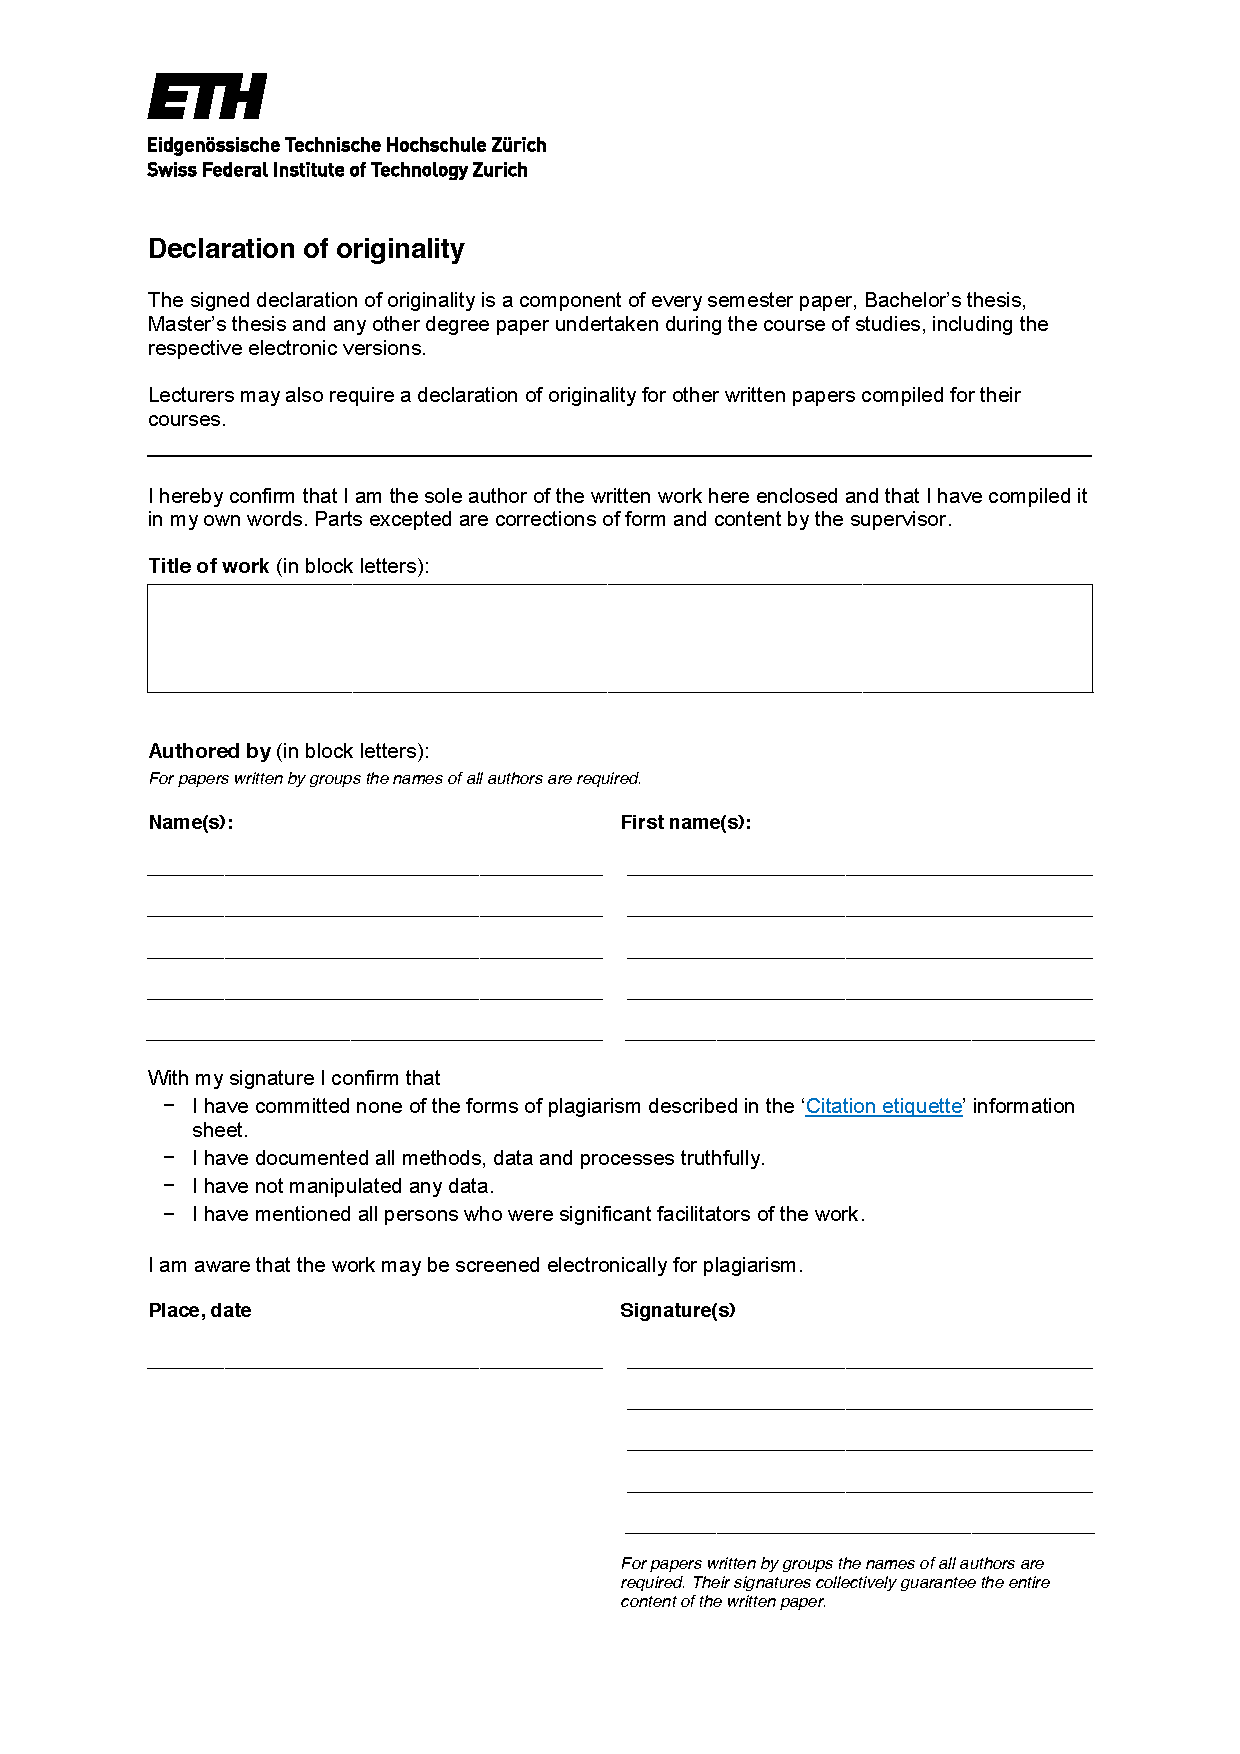
\includepdf[pages={-}]{declaration-originality.pdf}

\end{document}
